\chapter{Matrices simétricas y definidas positivas}\label{cap:sdp}

Este capítulo agrega una única condición a las matrices simétricas y recoge
una cantidad sorprendente de consecuencias. La condición es
\[
x^T S x > 0 \qquad \text{para todo } x \neq 0,
\]
y las matrices que la cumplen se llaman \emph{definidas positivas}. Es la
versión matricial de ``$s>0$'' para un número: así como un número positivo
tiene raíz cuadrada real, así como $s x^2$ es una parábola con un mínimo
estricto en el origen y así como dividir por $s$ nunca se traba, veremos que
una matriz sdp tiene raíz cuadrada, que $x^TSx$ tiene un mínimo estricto en el
origen y que la eliminación gaussiana nunca necesita permutar filas.

El capítulo es, en buena medida, una cosecha de lo que ya construimos. Del
Capítulo~\ref{cap:LU} usaremos los pivotes, la factorización $LDL^T$ y los
pivotes como cocientes de menores; del Capítulo~\ref{cap:schur}, el teorema
espectral $S=Q\Lambda Q^T$. El resultado central del capítulo dice que cinco
condiciones que provienen de esos lugares distintos --- una sobre la forma
cuadrática, una sobre los autovalores, una sobre la forma $A^TA$, una sobre
los determinantes y una sobre los pivotes --- son todas la misma condición.
Tener cinco caras de un mismo objeto es lo que vuelve a estas matrices tan
cómodas: uno elige la cara que más convenga según lo que tenga a mano.

No es un capítulo sólo teórico. Las matrices de covarianza son sdp (o al menos
semidefinidas) porque la varianza de cualquier combinación lineal de variables
no puede ser negativa; las matrices de Gram y las matrices \emph{kernel} lo son
por construcción; y en optimización las matrices sdp son exactamente las que
separan los problemas convexos, con mínimo global único, de los que tienen
mínimos locales y puntos de ensilladura. Volveremos a encontrarlas en los
capítulos de normas, de SVD y en el de mínimos cuadrados.

\section{Matrices simétricas y definidas positivas (sdp)}
\label{sec:sdp}

En los capítulos anteriores hemos trabajado extensamente con matrices
simétricas y ya establecimos para ellas varias propiedades fundamentales.
Recordemos, en primer lugar, que toda matriz simétrica tiene todos sus
autovalores reales y que sus autovectores correspondientes a autovalores
distintos son ortogonales entre sí. Más aún, el teorema espectral
(Teorema~\ref{teo:espectral-real}) nos permite afirmar que cualquier matriz
simétrica $S$ admite una descomposición $S = Q \Lambda Q^T$, donde $Q$ es
ortogonal --- sus columnas son una base ortonormal de autovectores --- y
$\Lambda$ es diagonal con los autovalores reales en la diagonal.

En el presente capítulo añadiremos una condición extra sobre estas matrices
simétricas. Esta condición resultará ser equivalente a que los autovalores en
la matriz diagonal $\Lambda$ sean todos positivos, y nos permitirá probar
otras caracterizaciones equivalentes de gran utilidad.

\begin{definition} Se dice que una matriz $A \in \R^{n\times n}$ es simétrica y
  definida positiva, o brevemente \textbf{sdp}, si
  \[
  A^T = A \qquad\text{y} \qquad x^T A x > 0, \quad \forall x \in \R^n\setminus\{0\}.
  \]
  Se dice \emph{semidefinida positiva} si $A^T=A$ y $x^T A x \ge 0$ para todo
  $x \in \R^n$.
\end{definition}

La cantidad $x^TAx$ se llama a veces la \textbf{energía} de $x$. Conviene
tenerla escrita como suma: si $A=(a_{ij})$,
\[
x^T A x = \sum_{i=1}^n\sum_{j=1}^n a_{ij}x_ix_j ,
\]
un polinomio homogéneo de grado $2$ en las variables $x_1,\dots,x_n$, que se
llama la \textbf{forma cuadrática} asociada a $A$. Por ejemplo, para
$A=\begin{bsmallmatrix} 2 & 1\\ 1 & 3\end{bsmallmatrix}$ resulta
$x^TAx = 2x_1^2 + 2x_1x_2 + 3x_2^2$.

\begin{remark}\label{obs:sdp-basicas} Vale la pena observar lo siguiente:
  \begin{enumerate}[label=\textbf{(\arabic*)}]
  \item
    $x^T A x = (Ax)\cdot x$. Luego, si $A$ es sdp el coseno del ángulo entre
    $Ax$ y $x$ es $>0$, por lo que el ángulo entre $x$ y $Ax$ es agudo. Si
    pensamos en la transformación $x \mapsto Ax$, vemos que transforma $x$ en
    otro vector $Ax$ que apunta en una dirección \emph{parecida} a $x$: ninguna
    matriz sdp da vuelta un vector.
  \item
    Si $A$ es sdp, entonces $A$ es invertible. En efecto, $Ax = 0$ implica
    $x^TAx=0$, lo que implica $x=0$; la única solución del problema homogéneo
    $Ax=0$ es la trivial.
  \item
    Si $A$ es sdp, $a_{ii} = e_i^T A e_i > 0$ para $i=1,\dots,n$: todos los
    elementos de la diagonal son positivos. (El recíproco es falso: en
    $\begin{bsmallmatrix} 1 & 10\\ 10 & 1\end{bsmallmatrix}$ la diagonal es
    positiva y $x=(1,-1)^T$ da energía $-18$.)
  \item
    Si $R \in \R^{m\times n}$, entonces $R^T R$ es simétrica y semidefinida
    positiva, pues $x^T R^T R x = (Rx)^T (Rx) = \|Rx\|^2 \ge 0$ para todo
    $x \in \R^n$. Si además las $n$ columnas de $R$ son linealmente
    independientes, entonces $R^T R$ es sdp (será necesario que $n \le m$).
  \item
    Si $A$ y $B$ son sdp y $t>0$, entonces $A+B$ y $tA$ son sdp: el conjunto
    de las matrices sdp es un \emph{cono convexo}. En cambio no es un
    subespacio, porque $-A$ nunca es sdp.
  \item
    Sabemos que toda matriz se puede escribir como suma de una simétrica más
    una antisimétrica:
    \[
    A = \underbrace{ \frac{A+A^T}2 }_{\text{parte simétrica de $A$}}
    + \underbrace{ \frac{A-A^T}2 }_{\text{parte antisimétrica de $A$}}.
    \]
    Como $x^T A x \in \R$, resulta $x^T A x = (x^T A x)^T = x^T A^T x$, y por
    lo tanto,
    \[ x^T \Big(\frac{A-A^T}2\Big) x = - x^T \Big(\frac{A-A^T}2\Big) x
    \quad \Longrightarrow \quad x^T \Big(\frac{A-A^T}2\Big) x = 0.
    \]
    En consecuencia
    \[
    x^T A x = x^T \Big(\frac{A+A^T}2\Big) x + x^T \Big(\frac{A-A^T}2\Big) x
    = x^T \Big(\frac{A+A^T}2\Big) x.
    \]
    Por lo tanto, si una matriz $A$ cumple $x^T A x > 0$ para todo
    $x \in \R^n\setminus\{0\}$, luego su \emph{parte simétrica}
    $\frac{A+A^T}2$ es sdp. Pedir simetría en la definición no es una
    restricción: la parte antisimétrica no se ve en la energía.
  \end{enumerate}
\end{remark}

\subsection{Tres ejemplos para tener a mano}
\label{sec:ejemplos-sdp}

Antes de probar nada conviene tener delante unas pocas matrices concretas. Las
tres que siguen van a reaparecer en todo el capítulo, y entre las tres cubren
los tres casos posibles: definida positiva, semidefinida, y simétrica pero
ninguna de las dos cosas.

\begin{example}[La matriz de las diferencias segundas]\label{ej:K}
Sea
\[
K=\begin{bmatrix} 2 & -1 & 0\\ -1 & 2 & -1\\ 0 & -1 & 2\end{bmatrix} .
\]
Es la matriz que aparece al discretizar una derivada segunda, y es
probablemente la matriz sdp más frecuente de toda la matemática aplicada. Que
es sdp se ve \emph{sin usar ningún teorema}, agrupando la energía en cuadrados:
\[
x^TKx = 2x_1^2+2x_2^2+2x_3^2-2x_1x_2-2x_2x_3
= x_1^2 + (x_1-x_2)^2 + (x_2-x_3)^2 + x_3^2 .
\]
Es una suma de cuadrados, así que $x^TKx\ge0$ siempre; y si vale $0$, los
cuatro cuadrados son nulos, lo que fuerza $x_1=0$, $x_1=x_2$, $x_2=x_3$, es
decir $x=0$. Luego $K$ es sdp.

Los cuatro cuadrados no aparecieron por casualidad. Son las cuatro
coordenadas de $Ax$, con
\[
A=\begin{bmatrix} 1&0&0\\ -1&1&0\\ 0&-1&1\\ 0&0&-1\end{bmatrix}
\in\R^{4\times3},
\qquad\text{y en efecto}\qquad A^TA=K .
\]
O sea que $x^TKx=\|Ax\|^2$: la matriz $K$ \emph{viene} escrita como $A^TA$,
que es el ítem~\ref{item-TeoEquivSDP-c} del teorema que vamos a probar. La
matriz $A$ toma diferencias de coordenadas consecutivas, y por eso a $K$ se la
llama matriz de diferencias segundas.
\end{example}

\begin{example}[La versión periódica: semidefinida]\label{ej:C}
Cambiemos las diferencias ``con bordes'' por diferencias \emph{cíclicas}: en
lugar de comparar $x_1$ con $0$ y $x_3$ con $0$, comparemos $x_3$ con $x_1$.
La matriz es
\[
C=\begin{bmatrix} 2 & -1 & -1\\ -1 & 2 & -1\\ -1 & -1 & 2\end{bmatrix} ,
\qquad
x^TCx = (x_1-x_2)^2 + (x_2-x_3)^2 + (x_3-x_1)^2 .
\]
Otra vez una suma de cuadrados, así que $x^TCx\ge0$: $C$ es semidefinida
positiva. Pero ahora la energía \emph{sí} se anula sin que $x$ sea cero: si
$x_1=x_2=x_3$ los tres cuadrados son nulos. Es decir,
$x^TCx=0$ para todo $x$ múltiplo de $(1,1,1)^T$, de modo que $C$ no es
definida positiva. De hecho $C(1,1,1)^T=0$: la matriz es singular, y sus
autovalores son $0$, $3$ y $3$.

La diferencia entre $K$ y $C$ es exactamente la diferencia entre ``definida''
y ``semidefinida'', y está en una sola cosa: si la suma de cuadrados puede
anularse sin que se anule $x$. Vale la pena quedarse con el ejemplo, porque es
el que explica de dónde salen las matrices semidefinidas: aparecen cuando el
problema tiene una \emph{simetría} ---acá, sumarle una constante a todas las
coordenadas no cambia nada--- y esa simetría se ve como un vector en el núcleo.
\end{example}

\begin{example}[Ser sdp no tiene nada que ver con tener entradas positivas]\label{ej:trampa}
Es el error más común. Comparemos
\[
P=\begin{bmatrix} 1 & 2\\ 2 & 1\end{bmatrix}
\qquad\text{y}\qquad
K_2=\begin{bmatrix} 2 & -1\\ -1 & 2\end{bmatrix} .
\]
Todas las entradas de $P$ son positivas, y sin embargo $P$ \emph{no} es sdp:
con $x=(1,-1)^T$ queda $x^TPx = 1-4+1=-2<0$. En cambio $K_2$ tiene entradas
negativas y sí es sdp: $x^TK_2x = x_1^2+(x_1-x_2)^2+x_2^2>0$ salvo en el
origen.

No hay ninguna contradicción: la energía $x^TSx$ mezcla las entradas con los
signos de las coordenadas de $x$, y por eso lo que importa no es el signo de
cada $a_{ij}$ sino el \emph{balance} entre la diagonal y lo que está fuera de
ella. Lo único cierto en esa dirección es lo que ya vimos en la
Observación~\ref{obs:sdp-basicas}(3): si $S$ es sdp, su diagonal es positiva.
El recíproco es falso, y $P$ es el contraejemplo.
\end{example}

\begin{remark}[Dónde aparecen de verdad]\label{obs:donde-aparecen}
Las tres de arriba son de juguete en el tamaño pero no en la forma. La que
aparece en los datos es la \textbf{matriz de covarianza}: si $X$ es una tabla
de datos con las columnas centradas, $S=\frac1{n-1}X^TX$ es semidefinida
positiva por la Observación~\ref{obs:sdp-basicas}(4), y es definida positiva
en cuanto las columnas de $X$ sean linealmente independientes. Es el objeto
central del Capítulo~\ref{cap:pca}, y toda la geometría de este capítulo
---la raíz cuadrada, las elipses, la distancia asociada a $S$--- se va a
aplicar ahí sin cambiar una coma.
\end{remark}

\subsection{El complemento de Schur de una matriz sdp}
\label{sec:schur-sdp}

Antes del teorema principal probamos un lema que usaremos dos veces: una para
los pivotes y otra para Cholesky. Recordemos de la
Sección~\ref{sec:schur-complemento} que si escribimos $A$ por bloques
\begin{equation}\label{eq:bloques-sdp}
A = \begin{bmatrix} \alpha & a^T \\ a & A_*\end{bmatrix},
\qquad \alpha\in\R,\quad a\in\R^{n-1},\quad A_*\in\R^{(n-1)\times(n-1)},
\end{equation}
y $\alpha\neq0$, entonces un paso de eliminación gaussiana deja
\[
\begin{bmatrix} \alpha & a^T \\ 0 & A_* - \tfrac1\alpha\, a a^T\end{bmatrix} ,
\]
y la matriz $A_* - \frac1\alpha a a^T$ es el \textbf{complemento de Schur} de
$\alpha$ en $A$. El lema dice que la condición sdp se hereda al complemento de
Schur; es decir, \emph{la eliminación gaussiana preserva la positividad}.

\begin{lemma}\label{lema:schur-sdp}
Sea $A\in\R^{n\times n}$ sdp, escrita por bloques como
en~\eqref{eq:bloques-sdp}. Entonces
\begin{enumerate}[label=\textbf{(\alph*)},itemsep=2pt,topsep=3pt]
\item $\alpha>0$ y $A_*$ es sdp;
\item el complemento de Schur $A_*-\frac1\alpha aa^T$ es sdp.
\end{enumerate}
\end{lemma}

\begin{proof}
(a) Ya vimos que $\alpha=a_{11}=e_1^TAe_1>0$. Y si $y\in\R^{n-1}$ es no nulo,
tomando $x=\begin{pmatrix}0\\ y\end{pmatrix}\neq0$ resulta
$y^TA_*y = x^TAx>0$; además $A_*$ es simétrica por serlo $A$.

(b) Sea $y\in\R^{n-1}$, $y\neq0$. La idea es elegir $\eta\in\R$ de modo que el
vector $x=\begin{pmatrix}\eta\\ y\end{pmatrix}$ tenga por energía exactamente
$y^T(A_*-\frac1\alpha aa^T)y$. Calculemos primero la energía de ese $x$:
\begin{align*}
x^T A x &= \begin{pmatrix}\eta & y^T \end{pmatrix}
\begin{bmatrix} \alpha & a^T \\ a & A_*\end{bmatrix}
\begin{pmatrix}\eta \\ y \end{pmatrix}
= \begin{pmatrix}\eta & y^T \end{pmatrix}
\begin{pmatrix} \alpha\eta+a^Ty \\ a\eta + A_*y\end{pmatrix}
\\
&= \alpha \eta^2 + \eta a^T y + \eta y^T a + y^T A_* y
= \alpha \eta^2 +2 \eta\, a^T y  + y^T A_* y.
\end{align*}
Por otro lado,
\[
y^T\Big(A_* - \tfrac1\alpha aa^T\Big) y
= y^T A_* y - \tfrac1\alpha (a^T y)^2 .
\]
Igualando las dos expresiones queda la ecuación
\[
\alpha \eta^2 + 2\eta\, a^Ty = -\tfrac1\alpha (a^Ty)^2,
\qquad\text{es decir}\qquad
\tfrac1\alpha\big(\alpha\eta + a^Ty\big)^2 = 0 ,
\]
que se cumple tomando $\eta = -\,a^Ty/\alpha$. Con esa elección,
$x\neq0$ (su cola es $y\neq0$) y por lo tanto
\[
y^T\Big(A_* - \tfrac1\alpha aa^T\Big) y = x^TAx > 0 .
\]
La simetría de $A_*-\frac1\alpha aa^T$ es inmediata.
\end{proof}

\begin{corollary}\label{coro:pivotes-positivos}
Si $A$ es sdp, la eliminación gaussiana sobre $A$ se puede llevar a cabo
\emph{sin intercambios de filas} y todos los pivotes resultan positivos.
\end{corollary}

\begin{proof}
El primer pivote es $\alpha=a_{11}>0$, así que el primer paso no se traba. Lo
que queda por eliminar después de ese paso es el complemento de Schur, que por
el Lema~\ref{lema:schur-sdp} vuelve a ser sdp y es de tamaño $n-1$. Por
inducción, su primer elemento diagonal --- que es el segundo pivote de $A$ ---
es positivo, y así sucesivamente.
\end{proof}

\subsection{Las cinco caracterizaciones}

\begin{theorem}\label{teo:equiv-sdp}
    Sea $S\in\R^{n\times n}$ una matriz simétrica. Las siguientes condiciones
    son equivalentes.
    \begin{enumerate}[label=\textbf{(\alph*)}]
        \item\label{item-TeoEquivSDP-a} $x^TSx>0$ para todo
          $x\in\R^n$ \emph{no nulo}.
        \item\label{item-TeoEquivSDP-b} Todos los autovalores de $S$ son positivos.
        \item\label{item-TeoEquivSDP-c} $S = A^TA$ para alguna matriz $A$ con
          columnas linealmente independientes.
        \item\label{item-TeoEquivSDP-d} Todos los determinantes principales
          $D_k=\det S_k$, $k=1,\dots,n$, son positivos.
        \item\label{item-TeoEquivSDP-e} Todos los pivotes de $S$ son positivos
          en la eliminación.
    \end{enumerate}
    (Aquí $S_k$ denota, como en el Capítulo~\ref{cap:LU}, la submatriz
    principal formada por las primeras $k$ filas y columnas de $S$.)
\end{theorem}

\begin{proof}
Probaremos el circuito
\[
\ref{item-TeoEquivSDP-a}\Rightarrow\ref{item-TeoEquivSDP-b}
\Rightarrow\ref{item-TeoEquivSDP-a},
\qquad
\ref{item-TeoEquivSDP-a}\Rightarrow\ref{item-TeoEquivSDP-e}
\Leftrightarrow\ref{item-TeoEquivSDP-d},
\qquad
\ref{item-TeoEquivSDP-e}\Rightarrow\ref{item-TeoEquivSDP-c}
\Rightarrow\ref{item-TeoEquivSDP-a}.
\]

\smallskip
\noindent\ref{item-TeoEquivSDP-a}$\Rightarrow$\ref{item-TeoEquivSDP-b}.
Sea $\lambda$ un autovalor de $S$ y $x\neq0$ un autovector correspondiente.
De $Sx = \lambda x$ sale $x^T S x = \lambda\, x^T x$, o sea
\[\lambda = \frac{x^T S x}{x^T x}.\]
El numerador es positivo por~\ref{item-TeoEquivSDP-a} y el denominador es
$\|x\|^2>0$. Luego $\lambda>0$.

\smallskip
\noindent\ref{item-TeoEquivSDP-b}$\Rightarrow$\ref{item-TeoEquivSDP-a}.
Por el teorema espectral (Teorema~\ref{teo:espectral-real}),
$S = Q \Lambda Q^T$ con $Q$ ortogonal y
$\Lambda = \diag(\lambda_1, \ldots, \lambda_n)$, donde $\lambda_i>0$ para todo
$i$ por~\ref{item-TeoEquivSDP-b}. Dado $x\neq0$, llamemos $y = Q^Tx$. Entonces
\[
x^TSx = x^TQ\Lambda Q^Tx = (Q^Tx)^T\Lambda (Q^Tx) = y^T\Lambda y
= \sum_{i=1}^n \lambda_i y_i^2 .
\]
Como $Q$ es invertible y $x\neq0$, es $y\neq0$, y entonces la suma es
estrictamente positiva.

\smallskip
\noindent\ref{item-TeoEquivSDP-a}$\Rightarrow$\ref{item-TeoEquivSDP-e}.
Es el Corolario~\ref{coro:pivotes-positivos}.

\smallskip
\noindent\ref{item-TeoEquivSDP-e}$\Leftrightarrow$\ref{item-TeoEquivSDP-d}.
Los dos sentidos salen de la fórmula de los pivotes como cocientes de menores
del Teorema~\ref{teo:LU}:
\[
u_{kk} = \frac{\det S_k}{\det S_{k-1}} = \frac{D_k}{D_{k-1}},
\qquad D_0:=1 .
\]
Si todos los pivotes son positivos, entonces
$D_k = u_{11}u_{22}\cdots u_{kk} > 0$ para todo $k$. Recíprocamente, si todos
los $D_k$ son positivos, cada $u_{kk}=D_k/D_{k-1}$ es cociente de dos números
positivos. (En ambos sentidos la hipótesis garantiza que los $D_k$ son no
nulos, así que las submatrices principales son invertibles y el
Teorema~\ref{teo:LU} se aplica: la eliminación no se traba.)

\smallskip
\noindent\ref{item-TeoEquivSDP-e}$\Rightarrow$\ref{item-TeoEquivSDP-c}.
Si los pivotes son no nulos, $S$ admite factorización $LU$ y, por ser
simétrica, la forma $S = LDL^T$ de la Sección~\ref{sec:LDU} con
$D=\diag(u_{11},\dots,u_{nn})$. Como todos los pivotes son positivos, tiene
sentido $D^{1/2}=\diag(\sqrt{u_{11}},\dots,\sqrt{u_{nn}})$ y podemos escribir
\[
S = L D L^T = \big(L D^{1/2}\big)\big(D^{1/2}L^T\big)
= A^T A, \qquad\text{con } A := D^{1/2}L^T .
\]
La matriz $A$ es triangular superior con diagonal $\sqrt{u_{kk}}\neq0$, luego
es invertible y sus columnas son linealmente independientes.

\smallskip
\noindent\ref{item-TeoEquivSDP-c}$\Rightarrow$\ref{item-TeoEquivSDP-a}.
Si $S=A^TA$ con $A\in\R^{m\times n}$ de columnas independientes, entonces para
$x\neq0$
\[
x^TSx = x^T(A^TA)x = (Ax)^T(Ax) = \|Ax\|^2 ,
\]
y $Ax\neq0$ porque $N(A)=\{0\}$. Luego $x^TSx>0$.
\end{proof}

\begin{remark}[Cuál usar]\label{obs:cual-usar}
Las cinco condiciones no cuestan lo mismo. Para decidir si una matriz concreta
es sdp, la condición~\ref{item-TeoEquivSDP-e} (los pivotes) es la más barata:
es una eliminación gaussiana, $\sim n^3/3$ operaciones, y de paso uno se queda
con la factorización. La~\ref{item-TeoEquivSDP-d} (los determinantes) es cómoda
a mano para $n=2$ o $3$ y desastrosa para $n$ grande. La~\ref{item-TeoEquivSDP-b}
(los autovalores) es la más cara de calcular pero la más informativa. La
\ref{item-TeoEquivSDP-a} es la definición, y la~\ref{item-TeoEquivSDP-c} es la
que aparece sola en las aplicaciones: las matrices de covarianza y las matrices
de Gram \emph{vienen} en la forma $A^TA$.
\end{remark}

\begin{example}\label{ej:sdp-2x2}
Para $n=2$ el criterio~\ref{item-TeoEquivSDP-d} es un renglón: $S =
\begin{bsmallmatrix} a & b\\ b & c\end{bsmallmatrix}$ es sdp si y sólo si
$a>0$ y $ac-b^2>0$. Así, $\begin{bsmallmatrix} 1 & 10\\ 10 &
100\end{bsmallmatrix}$ no es sdp ($D_2=0$: es semidefinida), mientras que
$\begin{bsmallmatrix} 1 & 10\\ 10 & 101\end{bsmallmatrix}$ sí lo es
($D_1=1>0$, $D_2=1>0$). Los pivotes de esta última son $1$ y
$101-100=1$, de acuerdo con $u_{22}=D_2/D_1$.
\end{example}

\begin{example}[Los cinco criterios, en una familia de matrices]\label{ej:equicorrelacion}
El teorema se aprecia mejor cuando hay un parámetro y la pregunta es ``¿para
qué valores?''. Tomemos
\[
S_b=\begin{bmatrix} 1 & b & b\\ b & 1 & b\\ b & b & 1\end{bmatrix} ,
\qquad b\in\R ,
\]
que no es una matriz inventada: es la matriz de correlación de tres variables
que están correlacionadas todas con todas por igual. La pregunta es para qué
$b$ es sdp, y vale la pena contestarla con tres criterios distintos para ver
que dan lo mismo y cuánto cuesta cada uno.

\medskip
\noindent\textbf{Con los autovalores (b).} Escribamos
$S_b=(1-b)I + b\,\mathbf 1\mathbf 1^T$, con $\mathbf 1=(1,1,1)^T$. Como
$\mathbf 1\mathbf 1^T$ tiene autovalor $3$ en la dirección $\mathbf 1$ y
autovalor $0$ en el plano $\mathbf 1^\perp$, los autovalores de $S_b$ son
\[
\lambda = 1+2b \ \ \text{(en la dirección } \mathbf 1),
\qquad
\lambda = 1-b \ \ \text{(doble, en } \mathbf 1^\perp).
\]
Los dos son positivos exactamente cuando
\[
\boxed{\ -\tfrac12 < b < 1\ }
\]

\medskip
\noindent\textbf{Con los determinantes (d).} Es una cuenta directa:
\[
D_1=1,\qquad D_2=1-b^2,\qquad D_3=\det S_b=(1-b)^2(1+2b) .
\]
Pedir los tres positivos da $-1<b<1$ de $D_2$, y $b>-\frac12$ con $b\neq1$ de
$D_3$; juntando todo, $-\frac12<b<1$. El mismo intervalo.

\medskip
\noindent\textbf{Con los pivotes (e).} Usando $u_{kk}=D_k/D_{k-1}$,
\[
u_{11}=1,\qquad u_{22}=1-b^2,\qquad u_{33}=\frac{(1-b)(1+2b)}{1+b} ,
\]
y de nuevo los tres son positivos exactamente en $-\frac12<b<1$.

\medskip
Tres observaciones que valen más que la cuenta.
\begin{itemize}[leftmargin=*,itemsep=2pt]
\item \emph{El intervalo no es simétrico.} Una correlación común puede ser
tan grande como se quiera (cerca de $1$) pero no puede ser muy negativa: con
$b<-\frac12$ la matriz deja de ser sdp. Tiene sentido: tres variables no
pueden estar todas muy anticorrelacionadas entre sí al mismo tiempo. Para
$n$ variables en lugar de tres, el mismo argumento da $-\frac1{n-1}<b<1$: el
margen negativo se achica a medida que hay más variables.
\item \emph{Los bordes son los casos semidefinidos.} En $b=1$ todas las filas
son iguales y $S_1=\mathbf 1\mathbf 1^T$ tiene rango uno; en $b=-\frac12$ el
autovalor $1+2b$ se anula y el núcleo es la dirección $\mathbf 1$ ---es,
salvo un factor, la matriz $C$ del Ejemplo~\ref{ej:C}---. Las matrices
semidefinidas son siempre el \emph{borde} del conjunto de las sdp.
\item \emph{Para qué sirvió cada criterio.} Acá los autovalores se pudieron
calcular porque la matriz tiene mucha simetría; es lo excepcional. En una
matriz cualquiera de $3\times3$ los autovalores son las raíces de una cúbica y
no hay fórmula cómoda, mientras que los determinantes y los pivotes siguen
siendo dos renglones. Esa es, en concreto, la asimetría de la
Observación~\ref{obs:cual-usar}.
\end{itemize}
\end{example}

\begin{entrega}{Matrices semidefinidas positivas}\label{ent:semidefinidas}
El Teorema~\ref{teo:equiv-sdp} tiene una versión ``con $\ge$'' que se usa tanto
como la original --- las matrices de covarianza son, en general, sólo
semidefinidas --- pero que no se obtiene cambiando mecánicamente $>$ por $\ge$
en las cinco condiciones. El objetivo es entender exactamente dónde falla.

Sea $S\in\R^{n\times n}$ simétrica.
\begin{enumerate}[label=\textbf{(\alph*)},itemsep=3pt,topsep=4pt]
\item Probar que son equivalentes: (i) $x^TSx\ge0$ para todo $x\in\R^n$;
(ii) todos los autovalores de $S$ son $\ge 0$; (iii) $S=A^TA$ para alguna
matriz $A$ (ahora sin pedir columnas independientes).
\emph{Sugerencia:} imitar el circuito
\ref{item-TeoEquivSDP-a}$\Rightarrow$\ref{item-TeoEquivSDP-b}$\Rightarrow$\ref{item-TeoEquivSDP-a}
del teorema y, para (iii), usar $A=\Lambda^{1/2}Q^T$.

\item Probar que $S$ es semidefinida positiva si y sólo si $S+\varepsilon I$ es
sdp para todo $\varepsilon>0$. Es decir: una matriz semidefinida se vuelve
definida apenas se le suma cualquier cosa positiva en la diagonal, por chica
que sea.

\item Mostrar con un ejemplo de $2\times2$ que la condición
``$D_k=\det S_k\ge 0$ para todo $k$'' \emph{no} implica que $S$ sea
semidefinida positiva.

\item El criterio correcto necesita \emph{todos} los menores principales y no
sólo los de arriba a la izquierda. Llamemos $S_{[I]}$ a la submatriz obtenida
quedándose con las filas y columnas de índices en $I\subseteq\{1,\dots,n\}$.
Probar que si $S$ es semidefinida positiva entonces $\det S_{[I]}\ge 0$ para
todo $I$. \emph{Sugerencia:} probar primero que $S_{[I]}$ es semidefinida
positiva, usando vectores $x$ con ceros fuera de $I$.

\item Explicar por qué el argumento del ítem (d) aplicado a las sdp da, gratis,
que $\det S_{[I]}>0$ para todo $I$, y en particular que en una matriz sdp vale
$a_{ij}^2 < a_{ii}a_{jj}$ para $i\neq j$. ¿Qué dice esto sobre dónde está el
elemento más grande en valor absoluto de una matriz sdp?

\item ¿Qué pasa con los pivotes de una matriz semidefinida positiva? Dar un
ejemplo en el que la eliminación se trabe y explicar qué se puede afirmar.
\end{enumerate}

\medskip
\noindent{\footnotesize\emph{Se entrega por escrito. El ítem (c) es el error
más frecuente con estas matrices; el (e) es la razón por la que en una matriz
de covarianza las varianzas ``dominan'' a las covarianzas. Dicho sea de paso,
el ítem (b) admite una lectura más corta para quien tenga a mano algo de
topología: dice que las matrices semidefinidas positivas son exactamente la
clausura del conjunto de las sdp.}}
\end{entrega}

\section{El cociente de Rayleigh}
\label{sec:rayleigh}

Las cinco caracterizaciones contestan la pregunta ``¿cuándo es la energía
$x^TSx$ positiva para todo $x$?''. La pregunta que sigue es la natural:
\emph{¿cuán grande puede ser esa energía?} Para que tenga sentido hay que
fijar el tamaño de $x$ ---si no, $x^TSx$ crece sin cota multiplicando $x$ por
un número grande---, y entonces la respuesta es exactamente el mayor
autovalor. Es el resultado más usado de todo el capítulo: con él se definen
los valores singulares en el Capítulo~\ref{cap:SVD}, se construyen las
componentes principales en el Capítulo~\ref{cap:pca} y se separan clases en el
Capítulo~\ref{cap:lda}.

Esta sección no usa nada más que el teorema espectral.

\begin{theorem}[El máximo de la energía sobre la esfera]\label{teo:rayleigh}
Sea $S\in\R^{n\times n}$ simétrica, con autovalores
$\lambda_1\ge\lambda_2\ge\cdots\ge\lambda_n$ y una base ortonormal de
autovectores $q_1,\dots,q_n$ (teorema espectral). Entonces, para todo $x$ con
$\|x\|=1$,
\[
\boxed{\ \lambda_n\ \le\ x^TSx\ \le\ \lambda_1\ }
\]
El máximo se alcanza en $x=q_1$ y el mínimo en $x=q_n$. Más precisamente, vale
$x^TSx=\lambda_1$ si y sólo si $x$ es un autovector unitario asociado a
$\lambda_1$.
\end{theorem}

\begin{proof}
\textbf{Paso 1: cambiar a la base de autovectores.} Sea
$Q=[\,q_1\ \cdots\ q_n\,]$, que es ortogonal, y $S=Q\Lambda Q^T$. Dado $x$,
llamemos $y=Q^Tx$, es decir, el vector de las coordenadas de $x$ en la base
$q_1,\dots,q_n$. Dos cuentas:
\[
x^TSx = x^TQ\Lambda Q^Tx = (Q^Tx)^T\Lambda(Q^Tx) = y^T\Lambda y
= \sum_{i=1}^n \lambda_i\,y_i^2 ,
\]
y, como $Q^T$ es ortogonal y por lo tanto no cambia las longitudes,
\[
\|y\| = \|Q^Tx\| = \|x\| = 1 ,
\qquad\text{o sea}\qquad
\sum_{i=1}^n y_i^2 = 1 .
\]
El problema quedó así: hay que acotar $\sum_i\lambda_iy_i^2$ sabiendo que
$\sum_i y_i^2=1$. Ya no hay matrices, sólo números.

\medskip
\textbf{Paso 2: la cota, restando.} En lugar de razonar sobre la suma, miremos
cuánto le falta para llegar a $\lambda_1$. Usando $\sum_iy_i^2=1$ para escribir
$\lambda_1 = \lambda_1\sum_iy_i^2$,
\[
\lambda_1 - x^TSx
= \lambda_1\sum_{i=1}^n y_i^2 - \sum_{i=1}^n \lambda_i y_i^2
= \sum_{i=1}^n (\lambda_1-\lambda_i)\,y_i^2 .
\]
Miremos un sumando cualquiera, $(\lambda_1-\lambda_i)\,y_i^2$. Es un producto
de dos números que \emph{no pueden ser negativos}: el primero porque
$\lambda_1$ es el mayor de todos los autovalores, y el segundo porque es un
cuadrado. Luego cada sumando es $\ge0$, y una suma de números $\ge0$ es $\ge0$.
Es decir, $\lambda_1-x^TSx\ge0$, que es la cota de arriba.

La de abajo es la misma cuenta del otro lado:
\[
x^TSx - \lambda_n = \sum_{i=1}^n (\lambda_i-\lambda_n)\,y_i^2\ \ge\ 0 ,
\]
porque ahora $\lambda_i-\lambda_n\ge0$ para todo $i$.

\medskip
\textbf{Paso 3: cuándo hay igualdad.} La cuenta del paso 2 da más que la
desigualdad: dice exactamente cuánto falta. Una suma de números $\ge0$ vale
cero si y sólo si \emph{todos} los sumandos son cero, así que
\[
x^TSx=\lambda_1
\iff (\lambda_1-\lambda_i)\,y_i^2=0 \ \text{ para todo } i
\iff y_i=0 \ \text{ para todo } i \text{ con } \lambda_i<\lambda_1 .
\]
Es decir, $x=Qy$ no tiene componente fuera del espacio propio de $\lambda_1$:
$x$ es un autovector unitario asociado a $\lambda_1$. En particular $x=q_1$
sirve, y da $q_1^TSq_1=\lambda_1$. Lo mismo para el mínimo con $\lambda_n$.
\end{proof}

\begin{remark}[Dónde está la gracia de la demostración]\label{obs:rayleigh-resta}
Conviene subrayar los dos movimientos, porque son los que hacen que el
argumento no requiera creer nada.

El primero es \emph{normalizar antes de empezar}: pedir $\|x\|=1$ convierte
una pregunta sobre un cociente en una pregunta sobre una suma con una
restricción, y las sumas con restricciones se manipulan sin esfuerzo.

El segundo es \emph{restar en lugar de comparar}. La tentación es decir que
$\sum_i\lambda_iy_i^2$ es un promedio ponderado de los $\lambda_i$ ---con
pesos $y_i^2$ que suman $1$--- y que un promedio nunca se sale del rango de
los números promediados. Es cierto, pero es una interpretación: para
convencerse hay que volver a hacer una cuenta. Restando, en cambio, la
desigualdad se vuelve una \emph{identidad}:
\[
\lambda_1 - x^TSx = \sum_{i=1}^n (\lambda_1-\lambda_i)\,y_i^2 ,
\]
y del lado derecho no hay nada que discutir: es una suma de productos de
números no negativos. De paso, la identidad entrega gratis el caso de
igualdad, que con el argumento del promedio hay que probar aparte.
\end{remark}

\begin{remark}[La lectura ``promedio ponderado'']\label{obs:rayleigh-promedio}
Dicho lo anterior, la lectura del promedio es la que deja la imagen correcta y
vale la pena tenerla, ahora que la cuenta ya está hecha. Los números
$w_i=y_i^2$ son no negativos y suman $1$, así que
\[
x^TSx=\sum_{i=1}^n \lambda_i w_i
\]
es una \emph{mezcla} de los autovalores. Por ejemplo, con
$\Lambda=\diag(5,2,1)$ y $x=\frac1{\sqrt3}(q_1+q_2+q_3)$ los pesos son
$w=(\frac13,\frac13,\frac13)$ y la energía vale $\frac{5+2+1}{3}=\frac83$, que
está entre $1$ y $5$ como tiene que estar.

Otra manera de verlo, útil para recordar \emph{dónde} se alcanza el máximo:
la condición $\sum_iy_i^2=1$ es un presupuesto de una unidad para repartir
entre las $n$ direcciones propias, y la dirección $i$-ésima paga $\lambda_i$
por cada unidad que se le asigne. Para cobrar lo máximo hay que poner todo el
presupuesto en la dirección que mejor paga, que es $q_1$; repartirlo entre
varias sólo puede empeorar el resultado. Eso explica por qué el máximo se
alcanza en un autovector y no en alguna dirección intermedia.
\end{remark}

El cociente que le da el nombre al resultado es sólo la manera de escribirlo
sin la restricción $\|x\|=1$.

\begin{definition}[Cociente de Rayleigh]\label{def:rayleigh}
Sea $S\in\R^{n\times n}$ simétrica. El \textbf{cociente de Rayleigh} de un
vector $x\neq0$ es
\[
R(x)=\frac{x^TSx}{x^Tx} .
\]
\end{definition}

\begin{corollary}[Versión con cociente]\label{coro:rayleigh-cociente}
Con la notación del Teorema~\ref{teo:rayleigh}, para todo $x\neq0$ vale
\[
\lambda_n\ \le\ \frac{x^TSx}{x^Tx}\ \le\ \lambda_1 ,
\qquad\text{es decir}\qquad
\max_{x\neq0}\frac{x^TSx}{x^Tx}=\lambda_1 ,
\quad
\min_{x\neq0}\frac{x^TSx}{x^Tx}=\lambda_n .
\]
\end{corollary}

\begin{proof}
Dado $x\neq0$, el vector $u=x/\|x\|$ tiene norma $1$, y
\[
R(x)=\frac{x^TSx}{\|x\|^2}
=\Bigl(\frac{x}{\|x\|}\Bigr)^{\!T}S\Bigl(\frac{x}{\|x\|}\Bigr)
=u^TSu ,
\]
así que el cociente de un $x$ cualquiera es la energía del vector unitario que
apunta en la misma dirección. Aplicando el teorema a $u$ se obtienen las dos
cotas, y los valores extremos se alcanzan en $q_1$ y $q_n$ como antes.
\end{proof}

\begin{remark}[Cuál de las dos formas usar]\label{obs:rayleigh-cual-usar}
Las dos dicen lo mismo y conviene tener las dos a mano, pero sirven para cosas
distintas. La forma con cociente es la cómoda para \emph{enunciar}, porque no
arrastra la condición $\|x\|=1$ y porque deja ver de un golpe que $R$ sólo
depende de la dirección de $x$: $R(cx)=R(x)$ para todo $c\neq0$. La forma con
la esfera, en cambio, es la cómoda para \emph{demostrar} y para \emph{calcular},
porque convierte el problema en maximizar una suma con una restricción.
Cuando haya que hacer una cuenta ---y en los capítulos que vienen las hay---
conviene normalizar primero y olvidarse del cociente.
\end{remark}

La versión restringida se demuestra sin cambiar nada: lo único que hace la
hipótesis extra es poner en cero algunas coordenadas $y_i$.

\begin{corollary}[Los autovalores siguientes]\label{coro:rayleigh-restringido}
Con la notación del Teorema~\ref{teo:rayleigh}, para cada $k=1,\dots,n$,
\[
\max\bigl\{\,x^TSx\ :\ \|x\|=1,\ x\perp q_1,\dots,q_{k-1}\,\bigr\}=\lambda_k ,
\qquad\text{alcanzado en } x=q_k .
\]
\end{corollary}

\begin{proof}
Con $y=Q^Tx$ como antes, la condición $x\perp q_i$ dice $y_i=q_i^Tx=0$. Si eso
vale para $i=1,\dots,k-1$, entonces
\[
x^TSx=\sum_{i\ge k}\lambda_i y_i^2 ,
\qquad \sum_{i\ge k} y_i^2 = 1 ,
\]
y repitiendo el Paso 2 con $\lambda_k$ en lugar de $\lambda_1$,
\[
\lambda_k - x^TSx = \sum_{i\ge k}(\lambda_k-\lambda_i)\,y_i^2\ \ge\ 0 ,
\]
porque $\lambda_i\le\lambda_k$ para $i\ge k$. La igualdad se alcanza en
$x=q_k$.
\end{proof}

\begin{remark}[Para qué lo vamos a usar]\label{obs:rayleigh-usos}
El teorema convierte un problema de autovalores en uno de \emph{optimización}:
$\lambda_1$ es el máximo de una función sobre la esfera, y $q_1$ el vector
donde se alcanza. De ahí salen las tres aplicaciones del resto del apunte.

\textbf{La norma espectral.} Dada $A\in\R^{m\times n}$ cualquiera ---ni
simétrica ni cuadrada---, ¿cuánto puede estirar a un vector? Con $\|x\|=1$,
\[
\|Ax\|^2=(Ax)^T(Ax)=x^T(A^TA)x ,
\]
y $A^TA$ es simétrica y semidefinida positiva
(Observación~\ref{obs:sdp-basicas}(4)). Por el teorema, ese máximo es
$\lambda_1(A^TA)$ y se alcanza en el autovector correspondiente. La raíz
cuadrada de ese número es el primer \emph{valor singular} de $A$ y también su
\emph{norma espectral}: es el punto de partida del Capítulo~\ref{cap:SVD}, y
notemos que para llegar ahí no hizo falta ninguna factorización nueva.

\textbf{De a una dirección por vez.} El
Corolario~\ref{coro:rayleigh-restringido} dice que $q_1$ maximiza, $q_2$
maximiza entre los perpendiculares a $q_1$, y así siguiendo. Esa construcción
secuencial es, literalmente, la definición de las componentes principales del
Capítulo~\ref{cap:pca}.

\textbf{Con dos matrices.} En el Capítulo~\ref{cap:lda} aparece el cociente
$x^TAx/x^TBx$ con $B$ sdp en el denominador. Se resuelve reduciéndolo a éste,
y la herramienta para hacerlo es la raíz cuadrada de $B$, que es el tema de la
sección que sigue.
\end{remark}

\begin{example}\label{ej:rayleigh-2x2}
Para $S=\begin{bsmallmatrix} 2 & 1\\ 1 & 2\end{bsmallmatrix}$ los autovalores
son $\lambda_1=3$, con $q_1=\frac1{\sqrt2}(1,1)^T$, y $\lambda_2=1$, con
$q_2=\frac1{\sqrt2}(1,-1)^T$. Evaluemos la energía en tres vectores unitarios:
\[
\begin{array}{llll}
x=q_1=\tfrac1{\sqrt2}(1,1)^T: & x^TSx=3=\lambda_1 & \text{(el máximo)} &
y=(1,0)^T,\\[2pt]
x=q_2=\tfrac1{\sqrt2}(1,-1)^T: & x^TSx=1=\lambda_2 & \text{(el mínimo)} &
y=(0,1)^T,\\[2pt]
x=(1,0)^T: & x^TSx=2 & \text{(en el medio)} &
y=\tfrac1{\sqrt2}(1,-1)^T.
\end{array}
\]
La tercera fila es la que ilustra la demostración: las coordenadas de
$(1,0)^T$ en la base de autovectores son $y=\frac1{\sqrt2}(1,-1)^T$, con pesos
$w=(\frac12,\frac12)$, y en efecto $3\cdot\frac12+1\cdot\frac12=2$. La cuenta
del Paso 2 da $\lambda_1-x^TSx=(3-3)\cdot\frac12+(3-1)\cdot\frac12=1$, que es
exactamente lo que le falta a $2$ para llegar a $3$.
\end{example}

\begin{entrega}{El cociente de Rayleigh}\label{ent:rayleigh}
Sea $S\in\R^{n\times n}$ simétrica, con $\lambda_1\ge\cdots\ge\lambda_n$ y
base ortonormal de autovectores $q_1,\dots,q_n$.

\begin{enumerate}[label=\textbf{(\alph*)},itemsep=3pt,topsep=4pt]
\item\label{item:rayleigh} \emph{(Otra demostración, sin coordenadas.)} Probar
el Teorema~\ref{teo:rayleigh} por un camino completamente distinto: mostrar
que los autovalores de $\lambda_1I-S$ son los $\lambda_1-\lambda_i$ y que por
lo tanto $\lambda_1I-S$ es semidefinida positiva; deducir de la condición de
la energía que $x^T(\lambda_1I-S)x\ge0$, es decir
$\lambda_1\,x^Tx\ge x^TSx$, para \emph{todo} $x$. Hacer lo mismo con
$S-\lambda_nI$ para la cota de abajo. ¿Cómo se identifican, en esta versión,
los vectores donde hay igualdad?

\item \emph{(Una familia, a mano.)} Sea
$S_c=\begin{bsmallmatrix} 2 & c\\ c & 2\end{bsmallmatrix}$ con $c\in\R$.
Calcular $\lambda_1(S_c)$ y $\lambda_2(S_c)$ y sus autovectores. Verificar el
teorema evaluando la energía en los vectores unitarios en las direcciones
$(1,0)$, $(1,1)$ y $(1,-1)$, y en cada caso escribir explícitamente los pesos
$w_i=y_i^2$ y la identidad del Paso 2. ¿Para qué valores de $c$ la dirección
de máxima energía deja de ser $(1,1)$?

\item \emph{(La traza, otra vez.)} Probar que
\[
\frac1n\sum_{i=1}^n q_i^TSq_i = \frac{\tr(S)}{n} ,
\]
y deducir que $\lambda_n\le \tr(S)/n\le\lambda_1$. Interpretar: el promedio de
la diagonal de $S$ siempre cae entre el menor y el mayor autovalor. Verificarlo
en las matrices $K$ y $C$ de los Ejemplos~\ref{ej:K} y~\ref{ej:C}.

\item \emph{(Hacia la norma espectral.)} Sea $A\in\R^{m\times n}$. Probar que
\[
\max_{\|x\|=1}\|Ax\|^2 = \lambda_1(A^TA) ,
\]
y que el máximo se alcanza en un autovector unitario de $A^TA$ asociado a
$\lambda_1$. Calcularlo explícitamente para
$A=\begin{bsmallmatrix} 3 & 0\\ 4 & 5\end{bsmallmatrix}$: hallar $A^TA$, sus
autovalores y el vector que más se estira, y comprobar el resultado
calculando $\|Ax\|$ en unos cuantos vectores unitarios.

\item \emph{(Monotonía.)} Probar que si $S$ y $T$ son simétricas y $T-S$ es
semidefinida positiva, entonces $\lambda_1(S)\le\lambda_1(T)$ y
$\lambda_n(S)\le\lambda_n(T)$. \emph{Sugerencia:} es inmediato con el
Teorema~\ref{teo:rayleigh}; ¿se le ocurre alguna demostración que no lo use?

\item \emph{(Opcional.)} Probar que el conjunto de valores que toma el
cociente de Rayleigh es exactamente el intervalo $[\lambda_n,\lambda_1]$:
todos los valores intermedios se alcanzan. \emph{Sugerencia:} mirar
$x(t)=(1-t)q_n+tq_1$ normalizado, con $t\in[0,1]$.
\end{enumerate}

\medskip
\noindent{\footnotesize\emph{Se entrega por escrito. El ítem (d) es, tal cual,
la definición del primer valor singular del Capítulo~\ref{cap:SVD}: conviene
hacerlo con cuidado porque se usa enseguida. El
Corolario~\ref{coro:rayleigh-restringido} es el primer caso de una familia de
resultados ---los teoremas de Courant-Fischer--- que describen \emph{todos}
los autovalores de una matriz simétrica como máximos y mínimos de la energía
sobre subespacios.}}
\end{entrega}

\section{La raíz cuadrada de una matriz sdp}
\label{sec:raiz}

La analogía con los números positivos se puede llevar bastante lejos. Si
$s>0$, existe un único $r>0$ con $r^2=s$. Lo mismo pasa con las matrices sdp,
y la construcción es inmediata a partir del teorema espectral: si
$S = Q\Lambda Q^T$ con $\Lambda=\diag(\lambda_1,\dots,\lambda_n)$ y todos los
$\lambda_i>0$, definimos
\[
\boxed{\ S^{1/2} := Q\,\Lambda^{1/2}\,Q^T,
\qquad \Lambda^{1/2}=\diag(\sqrt{\lambda_1},\dots,\sqrt{\lambda_n}).\ }
\]
Entonces $S^{1/2}$ es simétrica, sus autovalores $\sqrt{\lambda_i}$ son
positivos --- luego es sdp --- y
\[
\big(S^{1/2}\big)^2 = Q\Lambda^{1/2}Q^TQ\Lambda^{1/2}Q^T
= Q\Lambda^{1/2}\Lambda^{1/2}Q^T = Q\Lambda Q^T = S .
\]

\begin{remark}[Dos factorizaciones $S=A^TA$ distintas]\label{obs:dos-raices}
El Teorema~\ref{teo:equiv-sdp} nos dio una matriz $A$ con $S=A^TA$ y la
construcción anterior nos da otra: $S = S^{1/2}S^{1/2} = (S^{1/2})^TS^{1/2}$.
Son distintas --- una es triangular y la otra simétrica --- y ninguna de las
dos es la única: si $Q_0$ es cualquier matriz ortogonal, $A'=Q_0A$ cumple
$(A')^TA' = A^TQ_0^TQ_0A = A^TA = S$. Es decir, \emph{la factorización
$S=A^TA$ nunca es única}: la matriz $A$ está determinada a menos de una
ortogonal por izquierda. Lo que sí es único es el factor triangular con
diagonal positiva (Cholesky, próxima sección) y lo que sí es única es la
raíz \emph{sdp} (ítem (b) de la entrega que sigue).
\end{remark}

\begin{entrega}{La raíz cuadrada}\label{ent:raiz}
Sea $S\in\R^{n\times n}$ sdp y sea $S^{1/2}=Q\Lambda^{1/2}Q^T$ la matriz
construida más arriba.
\begin{enumerate}[label=\textbf{(\alph*)},itemsep=3pt,topsep=4pt]
\item Verificar que $S^{1/2}$ es sdp, que conmuta con $S$ y que
$S^{1/2}$ y $S$ tienen los mismos autovectores.

\item \emph{(Unicidad.)} Probar que $S^{1/2}$ es la \emph{única} matriz sdp
$R$ con $R^2=S$. \emph{Sugerencia:} si $R$ es sdp y $R^2=S$, y $v$ es un
autovector de $R$ con autovalor $\mu>0$, entonces $v$ es autovector de $S$ con
autovalor $\mu^2$; usar que la base de autovectores de $R$ diagonaliza también
a $S$ y que $\mu$ queda determinado por $\mu^2$ al ser $\mu>0$.

\item Mostrar que $\det(S^{1/2}) = \sqrt{\det S}$ y que
$\tr(S^{1/2}) = \sum_i\sqrt{\lambda_i}$. ¿Es cierto que
$\tr(S^{1/2})=\sqrt{\tr S}$? Dar un contraejemplo.

\item Exhibir una matriz simétrica $S$ y dos matrices \emph{simétricas}
distintas $R_1\neq R_2$ con $R_1^2=R_2^2=S$. ¿Se contradice el ítem (b)?

\item Calcular $S^{1/2}$ para $S=\begin{bsmallmatrix} 5 & 4\\ 4 &
5\end{bsmallmatrix}$ y para $S=\begin{bsmallmatrix} 10 & 6\\ 6 &
10\end{bsmallmatrix}$, y verificar en cada caso que
$(S^{1/2})^TS^{1/2}=S$.

\item Usando la raíz cuadrada, probar que si $S$ es sdp y $M$ es simétrica,
entonces $SM$ es diagonalizable y sus autovalores son reales, aunque $SM$
\emph{no} sea simétrica. \emph{Sugerencia:} $SM$ es semejante a
$S^{-1/2}(SM)S^{1/2} = S^{1/2}MS^{1/2}$, que sí es simétrica.
\end{enumerate}

\medskip
\noindent{\footnotesize\emph{Se entrega por escrito. El ítem (f) es la razón
por la que los problemas de autovalores generalizados $Ax=\lambda Bx$ con $B$
sdp se comportan como los simétricos; volveremos sobre eso más adelante.}}
\end{entrega}

\section{Factorización de Cholesky}
\label{sec:cholesky}

Entre todas las factorizaciones $S=A^TA$, hay una en la que $A$ es triangular
superior. Es la que efectivamente se calcula, porque cuesta la mitad que una
eliminación gaussiana común y porque resolver con factores triangulares es
inmediato.

\begin{theorem}\label{T:cholesky}
  Si $A \in \R^{n\times n}$ es sdp, entonces existe $R$ triangular superior
  (de $n\times n$) tal que $A = R^T R$.
\end{theorem}

\begin{proof}
  La demostración es constructiva. Observemos que si existiera tal matriz $R$
  debería cumplir que
  \[
  A = \begin{bmatrix} \alpha & a^T \\ a & A_*
  \end{bmatrix}
  = \begin{bmatrix} \rho & 0^T \\ r & R_*^T
  \end{bmatrix}
  \begin{bmatrix} \rho & r^T \\ 0 & R_*
  \end{bmatrix}
  =\begin{bmatrix} \rho^2 & \rho r^T \\ \rho r & R_*^T R_* + r r^T
  \end{bmatrix} ,
  \]
  con $\alpha = a_{11}$, $\rho \in \R$, $r \in \R^{n-1}$ y
  $A_*, R_* \in \R^{(n-1)\times (n-1)}$, con $R_*$ triangular superior.
  Para que valga la igualdad se debería cumplir:
  \begin{enumerate}
  \item $\rho^2 = \alpha$;
  \item $\rho r = a$;
  \item $R_*^T R_* + r r^T = A_*$.
  \end{enumerate}
  Para que se cumplan las dos primeras, basta con elegir
  $\rho = \sqrt{\alpha} > 0$ (recordemos que $\alpha = a_{11} > 0$) y
  $r = \frac1\rho a$. Para que se cumpla la tercera, observemos que debemos
  hallar $R_* \in \R^{(n-1)\times (n-1)}$, triangular superior, tal que
  \[
  R_*^T R_* = A_* - r r^T .
  \]
  Ahora bien, con la elección $r=a/\rho$ y $\rho^2=\alpha$ resulta
  \[
  A_* - rr^T = A_* - \tfrac1\alpha\, aa^T ,
  \]
  que es exactamente el complemento de Schur de $\alpha$ en $A$ y que, por el
  Lema~\ref{lema:schur-sdp}, es sdp. El argumento se sigue entonces por
  inducción sobre $n$ (el caso $n=1$ es $\rho=\sqrt{a_{11}}$).
\end{proof}

\begin{remark} Vale la pena observar lo siguiente:
  \begin{itemize}
  \item
    La matriz $R$ se llama \textbf{factor de Cholesky} de $A$.
  \item
    La factorización de Cholesky es una factorización $LU$ con $L=R^T$ y
    $U=R$ (aquí $L$ no tiene unos en la diagonal).
  \item
    Por el ítem~\ref{item-TeoEquivSDP-c} del Teorema~\ref{teo:equiv-sdp}, el
    recíproco también vale, de modo que podríamos haber enunciado el teorema
    de la siguiente manera:
    \begin{quote}
      Sea $A \in \R^{n\times n}$ simétrica. Entonces $A$ es sdp si y sólo si
      existe $R$ triangular superior no singular tal que $A = R^T R$.
    \end{quote}
  \item
    La demostración es un algoritmo: en cada paso se toma la raíz del primer
    elemento diagonal, se divide la primera fila por ella y se actualiza el
    bloque restante restándole $rr^T$.
  \end{itemize}
\end{remark}

\subsection*{Cuánto cuesta}

Contemos las operaciones como en la Sección~\ref{sec:conteo}, siguiendo los
pasos de la demostración. En el paso $k$-ésimo ($k=1,\dots,n$) el bloque
activo es de tamaño $(n-k+1)\times(n-k+1)$ y hay que hacer tres cosas:
\begin{enumerate}[label=\textbf{(\arabic*)},leftmargin=*,itemsep=2pt]
\item calcular $\rho=\sqrt{\alpha}$: \textbf{una raíz cuadrada};
\item calcular $r=a/\rho$, donde $a$ tiene $n-k$ componentes:
\textbf{$n-k$ divisiones};
\item actualizar el bloque restante, $A_*-rr^T$, que es de tamaño
$(n-k)\times(n-k)$.
\end{enumerate}
El paso (3) es el único que pesa, y es también donde aparece la ventaja de
Cholesky. La matriz $A_*-rr^T$ es simétrica, así que \emph{no hace falta
calcularla entera}: alcanza con su triángulo superior, que tiene
\[
\frac{(n-k)(n-k+1)}{2}
\]
entradas. Cada una de ellas cuesta una multiplicación (el producto
$r_ir_j$) y una resta. Ésa es exactamente la mitad del trabajo que hace la
eliminación gaussiana en el mismo paso, que actualiza las $(n-k)^2$ entradas
del bloque sin aprovechar la simetría.

Sumando sobre los $n$ pasos, el número total de multiplicaciones es
\[
\sum_{k=1}^{n}\frac{(n-k)(n-k+1)}{2}
=\sum_{m=0}^{n-1}\frac{m(m+1)}{2}
=\frac{(n-1)n(n+1)}{6}\ \approx\ \frac{n^3}{6},
\]
y el de restas es exactamente el mismo. Las $n$ raíces cuadradas y las
$\sum_k (n-k)=n(n-1)/2$ divisiones son de orden $n$ y $n^2$: no cuentan para
$n$ grande. En total,
\[
\frac{n^3}{6}+\frac{n^3}{6}=\frac{n^3}{3}\ \text{ operaciones},
\]
contra las $2n^3/3$ de la factorización $LU$ general que contamos en la
Sección~\ref{sec:conteo}: \textbf{Cholesky cuesta exactamente la mitad}.

El ahorro viene de dos lugares, y conviene separarlos. Primero, la simetría:
se guarda y se opera sobre medio arreglo. Segundo, y menos visible, el hecho
de que \emph{no hace falta buscar pivote}: por el
Teorema~\ref{teo:equiv-sdp}\ref{item-TeoEquivSDP-e} todos los pivotes de una
matriz sdp son positivos, así que la eliminación nunca se traba y nunca hay
que permutar filas. Eso no cambia el conteo de operaciones aritméticas, pero
sí evita las comparaciones y, sobre todo, los movimientos de datos, que en una
computadora real suelen costar más que las cuentas. Por las dos razones,
Cholesky es el algoritmo estándar para sistemas sdp, y de hecho la manera
práctica de \emph{verificar} que una matriz es sdp es intentar calcular su
factorización de Cholesky y ver si se traba al pedir una raíz cuadrada.

\begin{remark}[Unicidad]
  Dada $A$ sdp, existe una \emph{única} matriz $R$ triangular superior
  \emph{con elementos de la diagonal positivos} tal que $A = R^T R$: en la
  construcción anterior, la elección $\rho=+\sqrt\alpha$ es forzada en cada
  paso, y $r=a/\rho$ queda entonces determinado. Sin la condición sobre el
  signo hay $2^n$ factores, uno por cada elección de signos en la diagonal.
\end{remark}

\begin{remark}[Cholesky y $LDL^T$]
  Las dos factorizaciones son la misma cuenta escrita de dos maneras. Si
  $A=LDL^T$ es la factorización de la Sección~\ref{sec:LDU}, con $L$ de
  diagonal unitaria y $D$ la matriz de los pivotes (positivos por el
  Teorema~\ref{teo:equiv-sdp}), entonces
  \[
  A = LDL^T = \big(LD^{1/2}\big)\big(D^{1/2}L^T\big) = R^TR,
  \qquad R = D^{1/2}L^T ,
  \]
  y recíprocamente, si $A=R^TR$ y $D_R$ es la diagonal de $R$, entonces
  \[
  A = R^T R = \underbrace{R^T D_R\inv}_{L} \underbrace{D_R^2}_{D}
  \underbrace{D_R\inv R}_{L^T} .
  \]
  En particular, \emph{los elementos de la diagonal del factor de Cholesky son
  las raíces cuadradas de los pivotes}. Cholesky evita las raíces cuadradas
  sólo si uno se queda con $LDL^T$; ésa es la variante que se usa cuando $A$
  es sólo semidefinida.
\end{remark}

\section{La geometría: elipses y elipsoides}
\label{sec:elipses}

Hasta acá todo fue algebraico. La lectura geométrica es la que explica por qué
estas matrices aparecen en estadística y en optimización. Fijemos $S$ sdp y
miremos el conjunto de nivel
\[
E = \{x\in\R^n : x^TSx = 1\} .
\]

Empecemos por el caso diagonal. Si $S=\diag(\lambda_1,\dots,\lambda_n)$ con
$\lambda_i>0$, la ecuación es
\[
\lambda_1x_1^2 + \lambda_2x_2^2 + \cdots + \lambda_nx_n^2 = 1 ,
\]
es decir, una elipse (en $\R^2$), un elipsoide (en $\R^3$) o un elipsoide
$n$-dimensional, con \textbf{semiejes} sobre los ejes coordenados y de
longitudes $1/\sqrt{\lambda_1},\dots,1/\sqrt{\lambda_n}$: cuanto más grande el
autovalor, más corto el semieje.

El caso general se reduce a ése con el teorema espectral. Escribiendo
$S=Q\Lambda Q^T$ y llamando $y=Q^Tx$ --- que son las coordenadas de $x$ en la
base ortonormal de autovectores $q_1,\dots,q_n$ --- resulta
\[
x^TSx = y^T\Lambda y = \sum_{i=1}^n\lambda_i y_i^2 .
\]
Es la misma elipse de antes, vista en otra base ortonormal. Por lo tanto:

\begin{quote}
  \emph{El conjunto $x^TSx=1$ es un elipsoide cuyos ejes principales apuntan en
  las direcciones de los autovectores $q_i$ de $S$ y cuyos semiejes miden
  $1/\sqrt{\lambda_i}$.}
\end{quote}

Los autovectores dicen \emph{hacia dónde} está inclinada la elipse y los
autovalores dicen \emph{cuánto} mide en cada dirección. Que $S$ sea sdp es
justamente lo que garantiza que el conjunto de nivel sea acotado: si algún
$\lambda_i$ fuera negativo aparecería una hipérbola en vez de una elipse, y si
fuera cero, un cilindro.

\begin{example}
Para $S=\begin{bsmallmatrix} 3 & 1\\ 1 & 3\end{bsmallmatrix}$ los autovalores
son $\lambda_1=4$ y $\lambda_2=2$, con autovectores $q_1=(1,1)^T/\sqrt2$ y
$q_2=(1,-1)^T/\sqrt2$. La curva $3x_1^2+2x_1x_2+3x_2^2=1$ es entonces una
elipse inclinada $45^\circ$, con semieje corto $1/2$ en la dirección de
$(1,1)$ y semieje largo $1/\sqrt2$ en la dirección de $(1,-1)$
(Figura~\ref{fig:elipse}).
\end{example}

\begin{figure}[htbp]
\centering
\begin{tikzpicture}[scale=3.6,>=latex]
  % ejes
  \draw[->,gray!70] (-1.05,0) -- (1.05,0) node[below,black,font=\small] {$x_1$};
  \draw[->,gray!70] (0,-1.05) -- (0,1.05) node[left,black,font=\small] {$x_2$};
  % circunferencia unitaria de referencia
  \draw[gray!45,dashed] (0,0) circle (1);
  \node[gray!70,font=\scriptsize] at (0.80,0.80) {$\|x\|=1$};
  % elipse x^T S x = 1 con S=[[3,1],[1,3]]: semiejes 1/2 y 1/sqrt2, rotada 45
  \draw[very thick,blue!65!black,rotate=45] (0,0) ellipse (0.5 and 0.7071);
  \node[blue!65!black,font=\scriptsize,anchor=west] at (0.46,-0.52) {$x^TSx=1$};
  % ejes principales
  \draw[->,red!75!black,thick] (0,0) -- (0.3536,0.3536)
      node[midway,above left,font=\scriptsize,inner sep=1pt] {$\tfrac12$};
  \draw[->,red!75!black,thick] (0,0) -- (-0.5,0.5)
      node[midway,above right,font=\scriptsize,inner sep=1pt] {$\tfrac1{\sqrt2}$};
  \fill (0,0) circle (0.012);
  \node[red!75!black,font=\scriptsize] at (0.52,0.40) {$q_1$ ($\lambda_1=4$)};
  \node[red!75!black,font=\scriptsize] at (-0.60,0.66) {$q_2$ ($\lambda_2=2$)};
\end{tikzpicture}
\caption{La elipse $x^TSx=1$ para $S=\left[\begin{smallmatrix}3&1\\1&3\end{smallmatrix}\right]$.
Los ejes principales apuntan en las direcciones de los autovectores y los
semiejes miden $1/\sqrt{\lambda_i}$: el autovalor grande da el semieje corto.
En punteado, la circunferencia unitaria euclídea ($S=I$).}
\label{fig:elipse}
\end{figure}

Esta imagen es la que hay que tener en la cabeza en tres lugares distintos:

\begin{itemize}
\item en estadística, $E$ es una \emph{elipse de confianza}: si $\Sigma$ es la
matriz de covarianza de un vector aleatorio, $x^T\Sigma^{-1}x = c$ describe
las regiones de igual densidad de una gaussiana, y los autovectores de
$\Sigma$ son las direcciones de máxima y mínima varianza (esto es,
esencialmente, PCA);
\item en optimización, $E$ es un conjunto de nivel de la función que se
minimiza, y el cociente $\lambda_{\max}/\lambda_{\min}$ --- el
\emph{número de condición}, que veremos en el capítulo de normas de
matrices --- mide
cuán alargada es la elipse y, con eso, cuán lento es el descenso por gradiente;
\item en el Capítulo~\ref{cap:SVD} veremos que \emph{toda} matriz $A$ manda la
esfera unitaria a un elipsoide, y los semiejes de ese elipsoide serán los
valores singulares, que son las raíces de los autovalores de $A^TA$.
\end{itemize}

\begin{entrega}{Elipses, elipsoides y la distancia asociada a $S$}
\label{ent:elipses}
Sea $S\in\R^{n\times n}$ sdp, con autovalores
$\lambda_1\ge\cdots\ge\lambda_n>0$ y base ortonormal de autovectores
$q_1,\dots,q_n$. Para $x\in\R^n$ definimos
\[
\|x\|_S := \sqrt{x^TSx} .
\]
\begin{enumerate}[label=\textbf{(\alph*)},itemsep=3pt,topsep=4pt]
\item Probar que $\|x\|_S = \|S^{1/2}x\|$, donde $\|\cdot\|$ es la norma
euclídea usual y $S^{1/2}$ es la raíz cuadrada de la
Sección~\ref{sec:raiz}. Deducir que $\|x\|_S=0$ si y sólo si $x=0$, y que
$\|tx\|_S=|t|\,\|x\|_S$.

\item Probar las desigualdades
\[
\sqrt{\lambda_n}\,\|x\| \;\le\; \|x\|_S \;\le\; \sqrt{\lambda_1}\,\|x\| ,
\]
y mostrar que ambas se alcanzan (decir en qué vectores). \emph{Sugerencia:}
es el Teorema~\ref{teo:rayleigh} y nada más: $\|x\|_S^2=x^TSx$, así que para
$\|x\|=1$ las cotas son $\lambda_n$ y $\lambda_1$; el caso general sale
multiplicando por $\|x\|$. Interpretar: la ``regla'' $\|\cdot\|_S$ mide a lo
sumo $\sqrt{\lambda_1/\lambda_n}$ veces distinto que la euclídea.

\item Dibujar, para $S=\begin{bsmallmatrix} 4 & 0\\ 0 & 1\end{bsmallmatrix}$ y
para $S=\begin{bsmallmatrix} 5 & 4\\ 4 & 5\end{bsmallmatrix}$, el conjunto
$\{x : \|x\|_S=1\}$, indicando las direcciones y las longitudes de los
semiejes. Dibujar en el mismo gráfico la circunferencia unitaria euclídea.

\item Probar que $\langle x,y\rangle_S := x^TSy$ cumple las propiedades del
producto escalar que usamos en el Capítulo~\ref{cap:ortogonalidad}:
es bilineal, simétrico y $\langle x,x\rangle_S>0$ para $x\neq0$. Probar además
que $\|x\|_S^2 = \langle x,x\rangle_S$ y que vale la desigualdad de
Cauchy-Schwarz $|\langle x,y\rangle_S| \le \|x\|_S\|y\|_S$.
\emph{Sugerencia:} $\langle x,y\rangle_S = (S^{1/2}x)^T(S^{1/2}y)$ reduce todo
al caso euclídeo.

\item Dibujar la elipse $x^2+xy+y^2=1$ y calcular las longitudes de sus ejes a
partir de los autovalores de la matriz $S$ correspondiente. ¿Cuál es el área
encerrada? \emph{Sugerencia:} el área de una elipse de semiejes $a$ y $b$ es
$\pi ab$; expresarla en términos de $\det S$.

\item Sea $A\in\R^{m\times n}$ con columnas independientes y $S=A^TA$.
Probar que $\|x\|_S = \|Ax\|$. Interpretar geométricamente: la elipse
$\{x:\|x\|_S=1\}$ es la preimagen por $A$ de la esfera unitaria de $\R^m$.
\end{enumerate}

\medskip
\noindent{\footnotesize\emph{Se entrega por escrito. En el
Capítulo~\ref{cap:normas} veremos que $\|\cdot\|_S$ es un caso particular de
una noción general de norma, y que el producto $\langle\cdot,\cdot\rangle_S$
del ítem (d) es el ejemplo estándar de producto interno no euclídeo.}}
\end{entrega}

\section{Formas cuadráticas, mínimos y el Hessiano}
\label{sec:minimos}

\begin{remark}[Sobre esta sección]\label{obs:seccion-opcional}
Es la única del capítulo que usa cálculo en varias variables ---gradientes,
matrices Hessianas, desarrollo de Taylor de segundo orden---. Nada de lo que
viene después del capítulo depende de ella, así que puede leerse en diagonal,
o dejarse para el final, sin que eso afecte a la SVD, a las componentes
principales ni a nada de lo que sigue. Dicho esto, es la sección que explica
de dónde viene el nombre ``definida positiva'' y por qué estas matrices son
las que separan los problemas de optimización fáciles de los difíciles.
Quien no haya visto el Hessiano puede quedarse sólo con el
Teorema~\ref{teo:minimo-cuadratica}, cuya demostración es algebraica y no usa
derivadas en ningún lado.
\end{remark}

La otra lectura de las matrices sdp es la de la optimización, y es la que
justifica el nombre ``energía'' para $x^TSx$.

Empecemos por el caso más simple. Dada $S\in\R^{n\times n}$ simétrica y
$b\in\R^n$, consideremos
\[
J(x) = \tfrac12\, x^TSx - b^Tx ,
\]
que es la versión $n$-dimensional de $\frac12 sx^2-bx$. Si $S$ es sdp, esta
función tiene un mínimo global, es único y se calcula resolviendo un sistema
lineal.

\begin{theorem}\label{teo:minimo-cuadratica}
Sea $S\in\R^{n\times n}$ sdp y $b\in\R^n$. Entonces $J(x)=\frac12x^TSx-b^Tx$
tiene un único mínimo global, alcanzado en la solución $x^*$ de
\[
S x^* = b ,
\]
y el valor mínimo es $J(x^*) = -\frac12\,(x^*)^TSx^* = -\frac12\, b^TS^{-1}b$.
\end{theorem}

\begin{proof}
Como $S$ es invertible, $x^*=S^{-1}b$ está bien definido. Para cualquier
$x\in\R^n$ escribamos $x = x^*+h$. Usando $Sx^*=b$ y la simetría de $S$,
\begin{align*}
J(x^*+h) &= \tfrac12(x^*+h)^TS(x^*+h) - b^T(x^*+h)\\
&= \tfrac12 (x^*)^TSx^* + h^TSx^* + \tfrac12 h^TSh - b^Tx^* - b^Th\\
&= \underbrace{\tfrac12 (x^*)^TSx^* - b^Tx^*}_{J(x^*)}
 + \underbrace{h^Tb - b^Th}_{=\,0} + \tfrac12 h^TSh
= J(x^*) + \tfrac12\, h^TSh .
\end{align*}
Como $S$ es sdp, $h^TSh>0$ para todo $h\neq0$: el mínimo es estricto y único.
Finalmente, $J(x^*)=\frac12(x^*)^Tb - b^Tx^* = -\frac12 (x^*)^Tb$.
\end{proof}

\begin{remark}[Resolver un sistema es minimizar]\label{obs:sistema-minimizar}
El teorema se lee en los dos sentidos. De izquierda a derecha dice cómo
minimizar $J$: resolver $Sx=b$. De derecha a izquierda dice que resolver un
sistema con matriz sdp \emph{es} un problema de minimización, y por eso se le
pueden aplicar métodos de optimización. Ésa es la idea del método del
\emph{gradiente conjugado}, que es hoy el algoritmo estándar para sistemas sdp
grandes y ralos, donde la eliminación gaussiana es impracticable.
\end{remark}

Para funciones generales, la conexión pasa por la matriz de derivadas
segundas. Si $F:\R^n\to\R$ es dos veces derivable con continuidad, su
\textbf{matriz Hessiana} en un punto $x$ es
\[
H(x) = \begin{bmatrix}
\dfrac{\partial^2F}{\partial x_1^2} & \cdots & \dfrac{\partial^2F}{\partial x_1\partial x_n}\\[8pt]
\vdots & \ddots & \vdots\\[4pt]
\dfrac{\partial^2F}{\partial x_n\partial x_1} & \cdots & \dfrac{\partial^2F}{\partial x_n^2}
\end{bmatrix} ,
\]
que es simétrica porque las derivadas cruzadas coinciden. El desarrollo de
Taylor de segundo orden alrededor de un punto crítico $x_0$ (donde
$\nabla F(x_0)=0$) es
\[
F(x_0+h) = F(x_0) + \tfrac12\, h^T H(x_0)\, h + o(\|h\|^2) ,
\]
y ahí reaparece exactamente la forma cuadrática del
Teorema~\ref{teo:minimo-cuadratica}. De modo que el criterio de la derivada
segunda de una variable, $f''(x_0)>0$, se generaliza así:

\begin{center}
\begin{tabular}{ll}
\hline
$H(x_0)$ definida positiva & $x_0$ es un \textbf{mínimo} local estricto\\
$H(x_0)$ definida negativa & $x_0$ es un \textbf{máximo} local estricto\\
$H(x_0)$ con autovalores de ambos signos & $x_0$ es un \textbf{punto de ensilladura}\\
$H(x_0)$ singular semidefinida & el criterio no decide\\
\hline
\end{tabular}
\end{center}

\begin{example}
Para $F(x,y) = 4x^2+12xy+cy^2$ el Hessiano es constante,
$H = \begin{bsmallmatrix} 8 & 12\\ 12 & 2c\end{bsmallmatrix}$, y el origen es
un punto crítico. Los determinantes principales son $D_1=8>0$ y
$D_2=16c-144$. Entonces $(0,0)$ es un mínimo si $c>9$, un punto de
ensilladura si $c<9$, y para $c=9$ la matriz es semidefinida: la función es
$(2x+3y)^2$, que vale $0$ sobre toda una recta. El gráfico pasa de ser un bol
a ser una canaleta y después una montura.
\end{example}

\begin{entrega}{Mínimos y Hessianos}
\label{ent:minimos}
\begin{enumerate}[label=\textbf{(\alph*)},itemsep=3pt,topsep=4pt]
\item Calcular el gradiente de $J(x)=\frac12x^TSx-b^Tx$ con $S$ simétrica y
verificar que $\nabla J(x) = Sx-b$ y que el Hessiano de $J$ es $S$.
\emph{Sugerencia:} escribir $J$ en coordenadas y derivar respecto de $x_k$,
prestando atención a que $x_k$ aparece en la fila $k$ y en la columna $k$.

\item Probar que si $S$ es simétrica pero \emph{no} definida positiva,
entonces $J$ no tiene mínimo: exhibir una dirección $h$ en la que
$J(th)\to-\infty$ cuando $t\to\infty$. ¿Qué pasa si $S$ es semidefinida
positiva y singular?

\item Encontrar y clasificar los puntos críticos de
$F(x,y) = x^4+y^4-4xy$ usando el Hessiano. ¿En cuáles el criterio decide?

\item Sea $C\in\R^{m\times m}$ sdp y $A\in\R^{m\times n}$ con columnas
independientes. Probar que $S=A^TCA$ es sdp aplicando la condición de la
energía a $x^TA^TCAx$. (Esta matriz aparece en casi todos los métodos de
elementos finitos y en mínimos cuadrados con pesos.)
\end{enumerate}

\medskip
\noindent{\footnotesize\emph{Se entrega por escrito. El ítem (d) es la matriz
que aparece en casi todos los métodos de elementos finitos y en los problemas
de cuadrados mínimos con pesos.}}
\end{entrega}

\begin{remark}[Lo que queda para después]
Dos temas centrales quedan pendientes y tienen capítulo propio. El primero es
el problema de \textbf{mínimos cuadrados}: minimizar $\|Ax-b\|$ cuando el
sistema $Ax=b$ no tiene solución. Con lo de este capítulo ya están todas las
piezas --- la proyección del Capítulo~\ref{cap:ortogonalidad}, la matriz
$A^TA$ que ahora sabemos sdp cuando las columnas de $A$ son independientes, y
la factorización $QR$ ---, pero conviene tratarlo junto con sus variantes
(pesos, regularización, rango deficiente). El segundo es el de las
\textbf{normas} en general: acá apareció $\|x\|_S=\sqrt{x^TSx}$ como ejemplo,
y en el Capítulo~\ref{cap:normas} veremos qué tienen en común todas las
maneras razonables de medir.
\end{remark}

\section*{Ejercicios}

\begin{enumerate}

\item Muestre que si $S_1$ y $S_2$ son matrices sdp y $r>0$ entonces
\[rS_1 + S_2\]
 es una matriz sdp.
 
\item Suponga que $S^T=S$ y $S\bi{x}=\lambda\bi{x}$ y $S\bi{y}=\alpha\bi{y}$ son reales. Muestre que
$$
\bi{y}^T S\bi{x}=\lambda\bi{y}^T\bi{x}\quad\text{, }\quad\bi{x}^T S\bi{y}=\alpha\bi{x}^T\bi{y}\quad\text{y}\quad\bi{y}^T S\bi{x}=\bi{x}^T S\bi{y}.
$$
Además, muestre que $\bi{y}^T\bi{x}$ debe ser cero si $\lambda\neq\alpha$: \textbf{autovectores ortogonales.} \index{Ortogonal}

\item ¿\,Cuál o cuáles de $S_1$, $S_2$, $S_3$, $S_4$ tiene dos autovalores positivos\,? Use una condición, no calcule los $\lambda$. Encuentre también un $\bi{x}$ para el que $\bi{x}^T S_1 \bi{x} < 0$ y de este modo probar que $S_1$ no es definida positiva.
\[
S_1=\begin{bmatrix} 5&6\\ 6&7\end{bmatrix}\quad
S_2=\begin{bmatrix}  -1 & -2 \\  -2 &
    -5\end{bmatrix}\quad S_3=\begin{bmatrix} 1&10\\
  10&100\end{bmatrix} \quad S_4=\begin{bmatrix} 1&10\\
  10&101\end{bmatrix}.
\]

\item ¿\,Para qué números $b$ y $c$ las siguientes matrices son definidas positivas\,?
\[
S=\begin{bmatrix} 1&b\\ b&9\end{bmatrix}\qquad
S=\begin{bmatrix} 2&4\\ 4&c\end{bmatrix}\qquad
S=\begin{bmatrix} c&b\\ b&c\end{bmatrix}.
\]
Con los pivotes en $D$ y los multiplicadores en $L$, factorice cada $S$ en $LDL^T$.

\item He aquí una ``prueba'' rápida de que los autovalores de toda matriz real $A$ son reales\,:
\[
\textbf{Prueba falsa}\index{Prueba falsa}\quad
A\bi{x}=\lambda\bi{x}\quad\text{da}\quad \bi{x}^T A\bi{x}=\lambda\bi{x}^T \bi{x} \quad\text{así}\quad\lambda= \frac{\bi{x}^T A\bi{x}}{\bi{x}^T \bi{x}} = \frac{\text{real}}{\text{real}}.
\]
Encuentre la falla en este razonamiento, una suposición oculta injustificada. Puede seguir esos pasos con la matriz de rotación de $90^\circ$ $\begin{bmatrix}0 & -1\\ 1& 0\end{bmatrix}$ con $\lambda=i$ y $\bi{x}=(i,1)$.

\item Escriba $S$ y $B$ como $\lambda_1\bi{x}_1\bi{x}^T_1+\lambda_2 \bi{x}_2 \bi{x}^T_2$ del teorema espectral $Q\Lambda Q^T$:
\[
S = \begin{bmatrix} 3&1\\ 1&3\end{bmatrix} \qquad B =
\begin{bmatrix} 9&12\\ 12&16\end{bmatrix} \quad
\text{(mantenga } \|\bi{x}_1\|=\|\bi{x}_2\|=1\text{)}.
\]

\item (Recomendado) La siguiente matriz $M$ es antisimétrica\index{Antisimétrica} y también ortogonal.
Luego, todos sus autovalores son imaginarios puros y tienen $|\lambda|=1$. ($\|M\bi{x}\|=\|\bi{x}\|$ para todo $\bi{x}$ entonces $\|\lambda\bi{x}\|=\|\bi{x}\|$ para los autovectores.) Encuentre los cuatro autovalores a partir de la traza de $M$:
\[
M = \frac{1}{\sqrt 3}\begin{bmatrix} 0 & 1 & 1 & 1\\
    -1 & 0 &  -1 & 1\\   -1 & 1 & 0
  &  -1\\   -1 &   -1 & 1 &
0\end{bmatrix}\quad \text{solo puede tener autovalores } i \text{ o } -i.
\]

\item Muestre que la siguiente matriz $A$ (\textbf{simétrica pero compleja}) tiene solo una recta de autovectores:
\[
A = \begin{bmatrix} i&1\\ 1&-i\end{bmatrix} \; \text{no es ni siquiera diagonalizable: autovalores } \lambda=0 \text{ y }0.
\]
$A^T =A$ no es una propiedad especial para las matrices complejas. La buena propiedad es $\overline{A}^T = A$.  Entonces todos los autovalores son reales y $A$ tiene $n$ autovectores ortogonales.

\item Esta $A$ es casi simétrica pero sus autovectores están lejos de ser ortogonales:
\[
A=\begin{bmatrix}1 & 10^{-15}\\
0 & 1+10^{-15}
\end{bmatrix}\quad \text{tiene autovectores}\quad
\begin{bmatrix}1\\0\end{bmatrix}\quad \text{y}\quad
\begin{bmatrix}?\end{bmatrix}
\]
¿\,Cuál es el ángulo entre los autovectores\,?

\item \emph{¿\,Qué matrices simétricas $S$ también son ortogonales}\,? Las que tienen $S^T=S$ y $S^T=S^{-1}$.
\begin{itemize}
\item[(a)] Muestre cómo la simetría y la ortogonalidad llevan a $S^2=I$.
\item[(b)] ¿\,Cuáles son los autovalores posibles de $S$\,? Describa todos los $\Lambda$ posibles.
\end{itemize}
Entonces $S=Q\Lambda Q^T$ para una de esas matrices de autovalores $\Lambda$ y una $Q$ ortogonal.

\item Si $S$ es simétrica, muestre que $A^T SA$ también es simétrica (tome la traspuesta de $A^T SA$). Aquí $A$ es de $m \times n$ y $S$ es de $m\times m$. ¿\,Es cierto que los autovalores de $S$ coinciden con los de $A^T SA$\,?

\vspace{5pt}
\quad\; En caso de que $A$ sea cuadrada e invertible, se dice que $A^T SA$ es \emph{congruente} \index{Congruente} con $S$.

\quad\; Tienen la misma cantidad de autovalores positivos, negativos y cero: \textbf{Ley de inercia}\index{Ley de inercia}\index{Entrelazado/Entrelazamiento}.

\item He aquí una manera de mostrar que $a$ está \emph{entre} los autovalores $\lambda_1$ y $\lambda_2$ de $S$\,:

\vspace{-5pt}
$$
S=\left[\begin{array}{ll}
a&b\\
b&c\\
\end{array}\right]\qquad \begin{array}{l}
\det\,(S-\lambda I)=\lambda^2-a\lambda-c\lambda+ac-b^2\\
\text{es una parábola hacia arriba (debido a $\lambda^2$)}\\
\end{array}
$$

\noindent
Muestre que $\det\,(S-\lambda I)$ es negativa en $\lambda=a$. Entonces la parábola cruza el eje a la izquierda y a la derecha de $\lambda=a$. Lo cruza en los dos autovalores de $S$, que entonces deben encerrar a $a$.

Los $n-1$ autovalores de $A$ siempre se encuentran entre los $n$ autovalores de $S=\left[\begin{array}{@{\;}ll@{\;}}
A&\bi{b}\\
\bi{b}^T&c\\
\end{array}\right]$: es el fenómeno de \emph{entrelazado}\index{Entrelazado} de autovalores.

\item La energía $\bi{x}^T S\bi{x}=2x_1x_2$ tiene ciertamente un punto de ensilladura\index{Punto de ensilladura} y no un mínimo en $(0,0)$. ¿\,Qué matriz simétrica $S$ produce esta energía\,?\,¿\,Cuáles son sus autovalores\,?

\item Verifique alguna condición para ver si $A^T A$ es definida positiva en cada caso: $A$ necesita columnas independientes.
\[
A=\begin{bmatrix} 1&2\\ 0&3\end{bmatrix}\quad\text{o}\quad
A=\begin{bmatrix} 1&1\\ 1&2\\ 2&1\end{bmatrix} \quad\text{o}\quad
A=\begin{bmatrix} 1&1&2\\ 1&2&1\end{bmatrix}.
\]

\item Encuentre la matriz $S$ de $3$ por $3$ y sus pivotes, rango,
  autovalores, y determinante que satisface:
\[\begin{bmatrix} x_1 & x_2 & x_3\end{bmatrix}
     \begin{bmatrix}
       \vphantom{x_1}\\ \quad S\quad\vphantom{_1}\\
       \vphantom{x_1}\end{bmatrix}
       \begin{bmatrix} x_1\\
              x_2\\ x_3\end{bmatrix}
                =4(x_1-x_2+2x_3)^2.\]

\item Calcule los tres determinantes superiores izquierdos de $S$ para establecer si es definida positiva. Verifique que sus cocientes den el segundo y tercer pivote.
\[ \textbf{Pivotes $=$ cocientes de determinantes}\qquad
S=\begin{bmatrix} 2&2&0\\ 2&5&3\\ 0&3&8\end{bmatrix}.
\]

\item ¿\,Para qué números $c$ y $d$ son $S$ y $T$ definidas positivas\,?  Verifique sus $3$ determinantes\,:\linebreak
\[
S=\begin{bmatrix} c&1&1\\ 1&c&1\\ 1&1&c\end{bmatrix}\quad\text{o}\quad
T=\begin{bmatrix} 1&2&3\\ 2&d&4\\ 3&4&5\end{bmatrix}.
\]

\item Encuentre una matriz simétrica
\[ S=\begin{bmatrix}
  a&b\\ b&c
\end{bmatrix}
\]
cuyos elementos cumplan $a>0$, $c>0$ y $a+c>2b$, y que sin embargo tenga un
autovalor negativo. (Es decir: esas tres condiciones \emph{no} alcanzan para
que $S$ sea definida positiva.)

\item Una matriz definida positiva no puede tener un cero (o peor, un número negativo)\linebreak en su diagonal principal. Muestre que esta matriz no verifica $\bi{x}^T S \bi{x} > 0$:
\[\begin{bmatrix}x_1 & x_2 & x_3\end{bmatrix}
        \begin{bmatrix} 4&1&1\\ 1&0&2
        \\ 1&2&5  \end{bmatrix}
        \begin{bmatrix} x_1\\ x_2\\ x_3 \end{bmatrix}
        \text{ no es positiva cuando } (x_1,x_2,x_3)=(\quad
        ,\quad ,\quad ).
\]

\item Justifique el siguiente razonamiento: un elemento $s_{jj}$ de la diagonal
de una matriz simétrica $S$ no puede ser menor que \emph{todos} los autovalores
de $S$. En efecto, si lo fuera, $S-s_{jj}I$ tendría todos sus autovalores
positivos y sería definida positiva; pero $S-s_{jj}I$ tiene un cero en la
diagonal, lo que es imposible por el ejercicio anterior. Concluya que
$\lambda_{\min}\le s_{jj}\le\lambda_{\max}$ para todo $j$.

\item En la \index{Cholesky} factorización de Cholesky $S=A^T A$, con  $A=\sqrt{D}L^T$, las raíces cuadradas de los pivotes están en la diagonal de $A$. Encuentre $A$ (triangular superior) para
\[
S=\begin{bmatrix} 9&0&0\\ 0&1&2\\ 0&2&8\end{bmatrix} \quad\text{o}\quad
S=\begin{bmatrix} 1&1&1\\ 1&2&2\\ 1&2&7\end{bmatrix}.
\]

\item Sin multiplicar $S={\begin{bmatrix}
      \cos\theta & -\sin\theta\\ \sin\theta & \cos\theta\end{bmatrix}}
  {\begin{bmatrix} 2&0\\ 0&5\end{bmatrix}}
  {\begin{bmatrix} \cos\theta &
      \sin\theta\\  -\sin\theta & \cos\theta
    \end{bmatrix}}$,\; encontrar

\vspace{-9pt}
\begin{table}[h]
\begin{tabular}{ll}
(a) el determinante de $S$ & (b) los autovalores de $S$ \\ 
(c) los autovectores de $S$ & (d) una razón por la que $S$ es simétrica y definida positiva. \\
\end{tabular}
\end{table}

\item ¿\,Para cuáles $a$ y $c$ es esta matriz definida positiva\,? \, ¿\,Para cuáles $a$ y $c$ es semidefinida positiva (esto incluye definida)\,?

\index{$\bi{x}^T S\bi{x}$}
\vspace{-5pt}
$$
S=\left[\begin{array}{ccc}
a&a&a\\[3pt] a&a+c&a-c\\[3pt] a&a-c&a+c\\
\end{array}\right]\qquad \begin{array}{l}
\text{Las 5 condiciones son posibles.}\\[3pt]
\text{La energía } \bi{x}^T S\bi{x} \text{ es igual a}\\[3pt]
a\,(x_1+x_2+x_3)^2+c\,(x_2-x_3)^2.\\
\end{array}
$$

\end{enumerate}

%    \centerline{\bf Trabajo Pr\'actico 1}
%    \centerline{\bf Eliminación de Gauss y factorización LU.}

% \begin{pb}
%  Demostrar las siguientes afirmaciones:
% \begin{enumerate}[label=\textbf{(\alph*)}]
% \item Si $A$ y $B$ son matrices triangulares inferiores (unitarias) entonces $AB$ es triangular inferior (unitaria).
% \item Si $A$ es triangular inferior unitaria entonces $A$ es invertible y $A^{-1}$ es triangular inferior unitaria.
% \end{enumerate}
% %Demostrar las afirmaciones anteriores para matrices triangulares superiores teniendo en cuenta que la traspuesta de una matriz triangular superior es una matriz triangular inferior.
% \end{pb}

% \begin{pbstar}
%   Utilizar la funci\'on \verb+cputime+ de \ML para comparar los tiempos de ejecución de las funciones \verb+triinf+, \verb+triinf_filas+ y \verb+triinf_cols+ en la resolución de sistemas lineales con matrices triangulares inferiores. M\'as precisamente, considerar la resolución del sistema $Lx = b$, donde \verb+L = tril(reshape(1:N^2,N,N));+ y \verb+b = ones(N,1);+ para un $N$ dado. Comparar los tiempos de cpu para resolver dicho sistema con las tres funciones propuestas, graficando el tiempo de cpu invertido por cada una versus \verb+N = 20*2.^[3:10]+.
% \end{pbstar}

% \begin{pb}
%   Considerar la función \verb+triinf_cols+ para resolver sistemas triangulares inferiores, y basándose en esto, crear la función \verb+triinfM+ que resuelva varios sistemas simultáneamente. Más precisamente, si \verb+L+ es una matriz triangular inferior y \verb+b+ es una matriz cuyas columnas representan varios términos independientes, entonces \verb+x=triinfM(L,b)+ resuelve los distintos sistemas donde la $j$-ésima columna de \verb+x+ contiene la solución del sistema cuyo lado derecho es la $j$-ésima columna de \verb+b+.
% \end{pb}

% \begin{pb}
%   Basándose en la función \verb+triinf_cols+, crear la función \verb+trisup+ para resolver sistemas lineales de matrices triangulares superiores.
% \end{pb}
% % \item Notar que resolver \verb+LX=I+ donde \verb+L+ es triangular inferior e \verb+I+ es la matriz identidad equivale a encontrar la inversa de \verb+L+. Escribir una función \verb+X = TrinInfInv(L)+ para resolver este problema. Tratar de aprovechar el hecho de que el lado derecho es tan particular.

% \begin{pbstar}
%  Crear la función \verb+[l,u] = TridiLU(d,dmenos,dmas)+ que calcule la
%  factorización LU sin pivoteo de una matriz tridiagonal \verb+A+ donde
%  \begin{verbatim}
%    A = diag(dmenos(2:n),-1) + diag(d) + diag(dmas(1:n-1),1)
% \end{verbatim}
%  Los vectores \verb+l+ y \verb+u+ son tales que

% \begin{verbatim}
%    L = diag(ones(n,1)) + diag(l(2:n),-1)
%    U = diag(u) + diag(dmas(1:n-1),1)
% \end{verbatim}
%  Además:
% \begin{enumerate}[label=\textbf{(\alph*)}]
% \item Realizar el conteo de operaciones realizadas por \verb+TridiLU+ y comparar con la cantidad de operaciones realizadas por la función \verb+EleU+ desarrollada en clase.
% \item Crear las funciones \verb+TriInfBidi+ y \verb+TriSupBidi+ para resolver sistemas triangulares bidiagonales, donde los argumentos de entrada sean vectores.
% \item Considerar un sistema lineal asociado a la matriz $A$ de $N\times N$ ($N=100,1000,10000$) donde $$A=\begin{bmatrix}
% 2 & -1  &    &  &   &   \\
% -1 & 2  &-1   &  &   &   \\
%   & -1  & 2  &-1 &   &   \\
%   &    &    &\ddots &   &   \\
%      &    &  & -1 & 2 & -1\\
%      &    &  &   & -1 & 2 \\
%            \end{bmatrix}.$$
% \end{enumerate}
% Comparar los tiempos necesarios para hallar la solución del sistema utilizando las funciones \verb+EleU+, \verb+triinf_cols+ y \verb+trisup+ por un lado, y \verb+TridiLU+, \verb+TriInfBidi+ y \verb+TriSupBidi+ por otro lado.
% %\item Escribir una función que calcule la factorización LU de una matriz de Hessenberg. Realizar el conteo de operaciones. Comparar con la factorización LU que no aprovecha la forma particular de la matriz. Comparar a nivel experimental.

% \end{pbstar}

% \begin{pb}
%   Sean $g_j = (0 \ \ldots\  0\ m_{j+1,j}\  \ldots \ m_{n,j})^T$ para $j=1,2,\ldots,n-1$ vectores de Gauss. Sean $G_j := I-g_je_j^T$ las transformaciones de Gauss asociadas a $g_j$, $j=1,2,\ldots,n-1$.
%   Demostrar que:
%   \begin{enumerate}[label=\textbf{(\alph*)}]
%   \item $G_j^{-1} = I + g_je_j^T$, para $j=1,2,\ldots,n-1$.

%   \item $G_1^{-1}G_2^{-1}\ldots G_{n-1}^{-1}=I + \sum_{j=1}^{n-1} g_je_j^T$.
%   \end{enumerate}

% \end{pb}

% \begin{pb}
%  Demostrar que la matriz $A=\begin{bmatrix} 0 & 1 \\ 1 & 1 \end{bmatrix}$ no tiene una factorización LU.


% \end{pb}

% \begin{pbstar}
%   Considerar $\D A = \begin{bmatrix} \delta & 1 \\ 1 & 1 \end{bmatrix}$ y
%   $\D b = \begin{pmatrix} 1+\delta \\ 2\end{pmatrix}.$
%    \begin{enumerate}[label=\textbf{(\alph*)}]
%    \item Hallar la soluci\'on exacta de $Ax = b$  para $\delta\neq 1$.
%    \item Resolver el mismo sistema utilizando las funciones \texttt{EleU}, \verb+triinf_cols+ y \texttt{trisup}, para los
%   valores de $\delta = 10^{-2}, 10^{-4}, 10^{-6}, \dots, 10^{-18}$.
%   Armar una tabla de la forma
%   \begin{verbatim}
%    delta       x(1)      x(2)
%   -----------------------------
%    10^(-2)     xxxx      xxxx
%      .          .         .
%      .          .         .
%   \end{verbatim}
%    Explicar qu\'e sucede (Ayuda: pensar qu\'e ocurre con los errores de
%    redondeo al hacer la eliminaci\'on de Gauss.)
%    \end{enumerate}

% \end{pbstar}

% \begin{pbstar}
%  Resolver el sistema del ejercicio anterior utilizando la función \texttt{EleUpiv} en vez de \texttt{EleU}. Realizar la misma tabla y explicar qu\'e ocurre.

% \end{pbstar}

% \begin{pb}
%   Investigar c\'omo funciona la funci\'on \texttt{lu} de \ML. Comparar con la función \texttt{EleUpiv}.

% \end{pb}

% %    \centerline{\bf Trabajo Pr\'actico 2}
% %    \centerline{\bf Factorización de Cholesky. Factorización QR y }
% %



% \begin{pb}
%  % pag.405 B-F nuevo
% Demostrar que si una matriz $A\in\R^{n\times n}$ es \emph{estrictamente diagonalmente
% dominante} (e.d.d), es decir que sus elementos $a_{ij}$ verifican
% \[
% |a_{ii}| > \sum^n_{
% \begin{array}{c}
%   j=1 \\
%  j \neq i
% \end{array}} |a_{ij}|, \qquad i=1, 2, \ldots , n,
% \]
% entonces resulta ser no singular. ({\it Sugerencia:} Probar
%  que $Ax=0 \Rightarrow x=0$)


% \end{pb}

% \begin{pb}
%  % pag.405 B-F nuevo
% Demostrar que si $A$ es e.d.d., el sistema $Ax=b$ se puede resolver por
% Eli\-mi\-na\-ci\'on de Gauss sin intercambios de renglones.
% \end{pb}

% \begin{pb}

%   Una matriz cuadrada $A \in \R^{n\times n}$ se dice \emph{sim\'etrica y definida
%   positiva} (spd) si $A^T = A$ y satisface $x^T A x > 0$ para todo vector
%   $x \in \R^{n}$, $x \neq  0$. Decimos que es \emph{semi-definida positiva} si $x^T A x \ge 0$ para todo $x \in \R^{n}$.
%   Demostrar:
%   \begin{enumerate}[label=\textbf{(\alph*)}]
%   \item Si $R\in \R^{m\times n}$, entonces $R^TR$ es sim\'etrica y semi-definida positiva.
%   \item Si las columnas de $R\in \R^{m\times n}$ son linealmente independientes, entonces $R^T R$ es spd.
%   \item Si $A$ es spd, entonces
%   \begin{enumerate}[label=\textbf{(\roman*)}]
%   \item $A$ es invertible (o no singular).
%   \item Todos los autovalores de $A$ son positivos.
%   \item Los elementos de la diagonal de $A$ son positivos.
%   \item $a_{ij}^2 < a_{ii} a_{jj}$ para cada $i \neq j$.
%   \item $\max_{1 \le i, j \le n} |a_{ij}| \le
%   \max_{1 \le i \le n} |a_{ii}|$.
% \end{enumerate}



% \item Si $A$ es spd de orden $n$ y si la escribimos de la forma
%     \[
%       A = \begin{bmatrix}
%         \alpha & \quad & a^T & \quad \\
%         \\
%         a^T & \quad & A_* & \quad
%         \\
%         \end{bmatrix}
%     \]
%     con $\alpha \in \R$ y $A_*$ cuadrada de orden $n-1$, entonces $\alpha > 0$ y $A_*$
%     es spd.
%   \end{enumerate}

% \end{pb}

% \begin{pbstar}
%  Considerando las dos implementaciones propuestas para obtener la factorizaci\'on de Cholesky de una matriz, comparar el funcionamiento de ambas para factorizar matrices de diferentes ordenes de la
%       forma
%       \[
%       A = \begin{bmatrix}
%           \phantom{-}2 & -1 \\
%           -1 &  \phantom{-}2 & -1 & & 0\\
%              & -1 &  \phantom{-}2 & -1 \\
%              &    & \ddots & \ddots & \ddots \\
%              &  0  &        & -1 &  \phantom{-}2 & -1 \\
%              &    &        &   &  -1 & \phantom{-}2
%       \end{bmatrix}.
%   \]
% Sugerencia: Tenga en cuenta tanto los tiempos de cpu utilizados como los posibles l\'imites para la memoria requerida en ambos algoritmos.
% \end{pbstar}

% \begin{pbstar}
%  Realizar una funci\'on en \ML de nombre
%   \texttt{MinCuad(A,b)} que resuelva las ecuaciones normales
%   correspondientes al sistema $Ax=b$. ?`Qu\'e pasa si para un sistema
%   rectangular con m\'as filas que columnas escribimos \verb-A\b- en \ML?
%   Verificar y comparar el resultado arrojado por esta \'ultima
%   f\'ormula y el obtenido por la funci\'on \texttt{MinCuad(A,b)}.
%   Utilizando la funci\'on \texttt{help} de \ML indagar el
%   funcionamiento del s\'\i mbolo \verb-\- y de la funci\'on
%   \texttt{pinv} e informar brevemente.

% \end{pbstar}

% \begin{pb}
%  Supongamos que el precio de una casa depende principalmente de
%   dos variables: su edad ($x_1$) y el \'area de su superficie cubierta
%   ($x_2$) en metros cuadrados. Se propone el modelo lineal
%   \[
%   y  = \beta_0 + \beta_1 x_1 + \beta_2 x_2.
%   \]
%   Se observaron cinco casas seleccionadas aleatoriamente del mercado y
%   se obtuvieron los siguientes datos:
%   \begin{center}
%     \begin{tabular}{|c|c|c|}
%       \hline
%       Precio en   & Edad en        & Superficie cubierta          \\
%       miles ($y$) & a\~nos ($x_1$) & en m$^2 \times 100$ ($x_2$) \\
%       \hline
%       50  &   1  &  1 \\
%       40  &   5  &  1 \\
%       52  &   5  &  2 \\
%       47  &  10  &  2 \\
%       65  &  20  &  3 \\
%       \hline
%       \end{tabular}
%   \end{center}
%   Encontrar los valores de $\beta_0$, $\beta_1$, y $\beta_2$ que
%   minimizan el error por cuadrados m\'\i nimos. ?`Cu\'al es el error?
%   Estimar el costo de una vivienda de 25 a\~nos y 250~m$^2$ de
%   superficie cubierta.

% % \item
% %   Sea $Q \in \R^{n\times m}$ una matriz ortogonal (es decir $Q^TQ =
% %   I_m$). Demostrar que
% %   \[
% %   \left< Qx , Qy \right> = \left< x , y \right >
% %   \qquad\text{y} \qquad
% %   \| Qx \|_2 = \| x \|_2
% %   \qquad\forall x,y \in \R^m,
% %   \]
% %   donde $\left<\cdot,\cdot\right>$ denota el producto escalar en
% %   $\R^n$ o $\R^m$.

% \end{pb}

% % \begin{pb}
% %  Ortogonalización de Gram-Schmidt.
% %     \begin{enumerate}[{\bf (a)}]
% %     \item Describir el método de ortogonalización de Gram-Schmidt.
% %     \item Sea $A \in \R^{n\times k}$, con $n \ge k$ una matriz con columnas linealmente independientes.
% %     Demostrar que si se utiliza el método de ortogonalización de Gram-Schmidt
% %     con las columnas de $A$, entonces colocando los vectores de la nueva base
% %     como columnas de una matriz $Q$ se obtiene una descomposición $QR$ de $A$.
% %     \end{enumerate}
% %
% %
% % \end{pb}

%  \begin{pbstar}
%   Si $\{v_1,v_2,\dots,v_m\}$ son vectores linealmente independientes en $\R^n$ ($n\ge m$), y $\{u_1,u_2,\dots,u_m\}$ es el conjunto ortonormal obtenido por el proceso de ortogonalización de Gram-Schmidt, demostrar que
% \begin{equation*}
%   v_j\cdot u_j > 0,
% \end{equation*}
% para todo $j=1,2,\dots,m$.

%  \end{pbstar}


% {\color{red}{1-programar ortonormalizacion de vectores llii.}}

% \begin{pbstar}
%  Transformaciones de Householder
%       \begin{enumerate}[label=\textbf{(\alph*)}]
% %       \item Programar una función \texttt{[Q,R] = qrHouse(A)} que obtenga la
% %       descomposición $QR$ de la matriz $A$ utilizando las transformaciones de
% %       Householder. Las columnas de la matriz $Q$ deberán ser los vectores $u$ de las
% %       transformaciones de Householder que logran la factorización.
% %
% %       \item Programar una función \texttt{[x,e] = qrSolve(Q,R,b)} que resuelva el
% %       problema de cuadrados mínimos correspondiente al sistema $Ax=b$, donde $Q$ y $R$
% %       son las matrices que produce \texttt{qrHouse}. El vector de salida \texttt{x}
% %       debe contener la soluci\'on, y el número \texttt{e} debe contener la norma del
% %       residuo $Ax-b$ (!`sin calcularlo de esta forma!, sino de manera eficiente).

%       \item Programar una función \texttt{[x,e] = MinCuadQR(A,b)} que resuelva el
%       problema de cuadrados mínimos correspondiente al sistema $Ax=b$, utilizando las
%       dos funciones \texttt{[U,R] = qrhouse(A)} y \texttt{[x,e] = qrsolve(U,R,b)} vistas en clase.

%       \item Utilizando la función \texttt{MinCuadQR(A,b)}, crear la función \texttt{a = ajustar(x,y,n)} que reciba como
%       argumentos:
%       \begin{itemize}
%       \item[] \texttt{x, y}: coordenadas de puntos a ajustar con un polinomio.
%       \item[] \texttt{n}: grado del polinomio con el que se ajustarán los puntos.
%       \end{itemize}
%       La salida deben ser los coeficientes del polinomio obtenido, donde
%           \texttt{a(1)} es el coeficiente de orden \texttt{n},
%           \texttt{a(2)} el de orden \texttt{n-1}, y así sucesivamente, hasta
%           \texttt{a(n+1)} que es el coeficiente de orden cero.
%       \end{enumerate}
%       %En todas las funciones programadas se debe tener en cuenta la \emph{eficiencia}.
% \item Realizar el conteo de operaciones necesarias para resolver el problema de mínimos cuadrados asociado al sistema $Ax=b$ con $A\in\R^{n\times k}$ con $n$ mucho mayor que $k$ mediante:
% \begin{enumerate}[label=\textbf{(\alph*)}]
%  \item El \emph{método de las ecuaciones normales}, es decir, resolviendo el sistema $A^T A x= A^T b$ mediante la descomposición de Cholesky.
% \item La descomposición QR de $A$ utilizando el método de Gram-Schmidt.
% \item La descomposición QR de $A$ utilizando las transformaciones de Householder (función \texttt{[x,e] = MinCuadQR(A,b)}).
% \end{enumerate}

% \end{pbstar}

% \begin{pbstar}
%  Analizar experimentalmente la velocidad y la precisión (o estabilidad) de las funciones \texttt{MinCuad(A,b)}, \texttt{MinCuadQR(A,b)} y \texttt{$\backslash$} (de \ML) al resolver el siguiente problema de mínimos cuadrados:
% $Ax=b$ donde $A\in\R^{n\times 4}$ es la matriz $$\verb+A = [a.^3, a.^2, a, ones(n,1)]+$$ para \verb+a = linspace(1,5,n)'+, y el vector $b$ elegido de manera que la solución exacta del problema sea $x=(1, 1, 1, 1)^T$. Considerar distintos valores grandes de $n$.
% \end{pbstar}


